\chapter{Models for Light Curve Classification}


\section{Introduction}

Our goal is to develop a model for the classification of stellar variability, capable of distinguishing variable stars from non-variable stars and categorizing variable stars into their respective classes.

Since distinguishing between variable and non-variable stars and classifying variable stars into their specific variability types are related but fundamentally different tasks, we adopt a hierarchical classification approach.

\begin{itemize}
    \item \textbf{Task A.} Classify stars as \textbf{variable} or \textbf{non-variable}.
    \item \textbf{Task B.} Classify stars identified as variable into their respective variability types - \textbf{pulsating}, \textbf{rotating}, \textbf{eclipsing}.
\end{itemize}


\section{Training Dataset}

We constructed a training dataset for both tasks by preprocessing the available light curves and further remapped the labels shown in \hyperref[tab:05_base_class_counts]{Table 5.1}.

\subsection{Parameters}

The following parameters were used for the preprocessing.

\begin{table}[H]
    \centering
    \scriptsize
    \renewcommand{\arraystretch}{1.2}
    \begin{tabularx}{\textwidth}{X c}
        \toprule
        \textbf{Parameter} & \textbf{Value} \tabularnewline
        \midrule
        TARGET\_LENGTH & $256$ \tabularnewline
        STANDARDIZE\_FLUX & True \tabularnewline
        CREATE\_SEGMENTS & True \tabularnewline
        MIN\_RAW\_POINTS\_PER\_SEGMENT    & $4096$ \tabularnewline
        SEGMENT\_STRIDE\_RAW\_POINTS  & $4096$ \tabularnewline
        OUTLIER\_SIGMA & $5$ \tabularnewline
        \bottomrule
    \end{tabularx}
    \caption[Preprocessing Configuration]{Preprocessing Configuration}
    \label{tab:06_preprocessing_configuration}
\end{table}

\FloatBarrier

\subsection{Task A Dataset}

The dataset for Task A is well-balanced, contains only two classes and is also quite large with no marginalized class which should make it the easier of the two tasks.

\begin{table}[H]
    \scriptsize
    \centering
    \renewcommand{\arraystretch}{1.3}
    \begin{tabularx}{\textwidth}{Xcccc}
        \toprule
        \textbf{Class (Label)} & \textbf{Original Label} & \textbf{TIC Count} & \textbf{TIC Total} & \textbf{Segment Total}  \tabularnewline \midrule
        Non-Variable (\textbf{N}) & Non-Variable & \num{1729} & \num{1729} & \num{57262}   \tabularnewline \midrule
        Variable (\textbf{V}) &
        \begin{tabular}{@{}c@{}}
            Unspecified-Variable \\ Pulsating \\ Rotating \\ Eclipsing
        \end{tabular} &
        \begin{tabular}{@{}c@{}}
            720 \\ 535 \\ 262 \\ 101
        \end{tabular} & \num{1618} & \num{56093} \tabularnewline \midrule
        Total & & & \num{3347} & \bfseries{\num{113355}} \tabularnewline
        \bottomrule
    \end{tabularx}
    \caption[Task A Dataset]{Task A Dataset}
    \label{tab:06_task_a_data}
\end{table}

\FloatBarrier

\subsection{Task B Dataset}

The dataset for Task B is on the other hand significantly smaller and contains 3 imbalanced classes, with the Eclipsing (\textbf{E}) class having only $101$ individual TICs.

\begin{table}[H]
    \scriptsize
    \centering
    \renewcommand{\arraystretch}{1.3}
    \begin{tabularx}{\textwidth}{Xcccc}
        \toprule
        \textbf{Class (Label)}           & \textbf{Original Label}    & \textbf{TIC Count} & \textbf{TIC Total} & \textbf{Segment Total}       \tabularnewline \midrule
        Pulsating (\textbf{P})   & Pulsating         & 535   & 535    & \num{17868}          \tabularnewline
        Rotating (\textbf{R})    & Rotating          & 262   & 262    & \num{9806}          \tabularnewline
        Eclipsing (\textbf{E})   & Eclipsing         & 101   & 101    & \num{3176}                 \tabularnewline \midrule
        Total           & & & 898       & \num{30850}          \tabularnewline
        \bottomrule
    \end{tabularx}
    \caption[Task B Dataset]{Task B Dataset}
    \label{tab:06_task_b_data}
\end{table}

\FloatBarrier

Each proposed model configuration was then trained and evaluated on both tasks.


\section{Methodology}

\subsection{Protocol}

The standard \textbf{train} / \textbf{val} / \textbf{test} protocol was again adopted, with the \textbf{test} set used only for the evaluation of the one final model.
We have also experimented with $k$-fold \textbf{cross-validation}, however its implementation using the transformers library proved cumbersome, the training time has grown significantly ($\approx k$ times) and the performance wasn't noticeably better when compared to the alternative train/val/test protocol.

\subsection{Metrics and Evaluation}

Model performance was evaluated at both the segment level and the TIC level.
Although the model is trained on individual light-curve segments, the scientific target is the classification of the underlying TIC object (star).

For this reason, segment-level metrics were only used for training and to monitor the behavior of the model on individual input samples, while TIC-level metrics computed during validation stage were used as the primary criterion for model selection.
TIC-level classification would also be applied in real-world labeling of unknown stars.

\begin{figure}[!htbp]
    \centering
    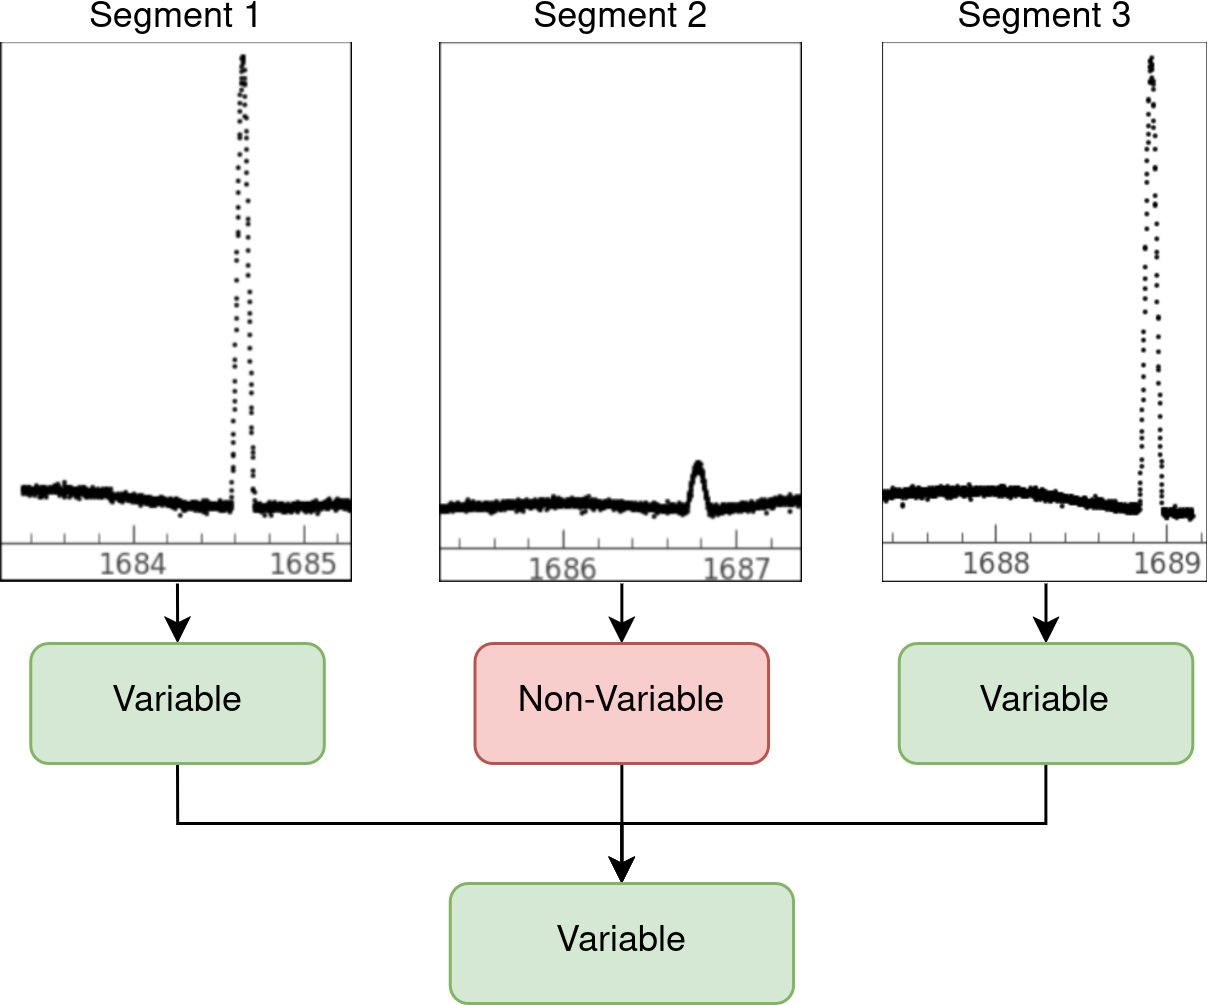
\includegraphics[width=0.8\linewidth]{images/06/segment_vs_tic_classification}
    \caption[Segment vs. TIC classification]{Comparison of segment-level and TIC-level classification - while one of the segments would individually misclassify the star, the final TIC-level prediction is correct. Note that the TIC-level prediction isn't done by majority voting, but rather by averaging logits.}
    \label{fig:06_segment_vs_tic_classification}
\end{figure}

\subsubsection{Segment \& Class Weighted Loss}\label{subsubsec:06-turbo-loss}

During training and validation, the loss was computed as a segment and class-weighted segment-level cross-entropy loss.
For a batch of segments, the model produces logits for each segment, and cross-entropy is computed independently for each one.
Class weights were applied inside the cross-entropy term to account for class imbalance.
To prevent TICs with many extracted segments from dominating, each segment was additionally weighted by the inverse of the number of segments belonging to its TIC.
Therefore, for segment $i$ from TIC $t$, the segment weight is

\[
    s_i = \frac{1}{n_t},
\]

where $n_t$ is the number of segments associated with TIC $t$.
The batch loss is then computed as the weighted average

\[
    \mathcal{L} = \frac{\sum_{i=1}^{B} s_i \, L_{\mathrm{WCE}}^{(i)}}{\sum_{i=1}^{B} s_i},
\]

where $B$ is the batch size and $L_{\mathrm{WCE}}^{(i)}$ is the \hyperref[eq:04-weighted-cross-entropy]{WeightedLoss} for segment $i$.

\bigskip

\noindent With this improvement, the training objective remained segment-based, but TIC-aware weighing ensured that each TIC contributed approximately equally to the loss.

\subsubsection{TIC-level Metrics}

The validation loss was computed at the end of each epoch using the same weighted segment-level cross-entropy objective as in training.

However, since we are interested in the model's performance on TIC level rather than the segment level, an additional TIC-level evaluation was performed during validation.

For each validation segment $i$ belonging to TIC $t$, the model output logits

\[
    \mathbf{z}_{t,i} = [z_{t,i,1}, z_{t,i,2}, \dots, z_{t,i,C}],
\]

where $C$ is the number of classes.
These logits were converted to class probabilities using the softmax function

\[
    p_{t,i,c} = \frac{\exp(z_{t,i,c})}{\sum_{k=1}^{C} \exp(z_{t,i,k})}.
\]

The class probabilities were then averaged over all $n_t$ segments belonging to the same TIC

\[
    \bar{p}_{t,c} = \frac{1}{n_t} \sum_{i=1}^{n_t} p_{t,i,c}.
\]

The predicted class for TIC $t$ was selected as the class with the highest mean probability

\[
    \hat{y}_t = \arg\max_{c} \bar{p}_{t,c}.
\]

Equivalently

\[
    \hat{y}_t = \arg\max_c \left(\frac{1}{n_t}\sum_{i=1}^{n_t}\mathrm{softmax}(\mathbf{z}_{t,i})_c\right).
\]

After aggregation, we obtained exactly one predicted label for each TIC.
TIC-level accuracy was then computed as

\[
    \mathrm{Accuracy}_{\mathrm{TIC}} = \frac{1}{T} \sum_{t=1}^{T} \mathbf{1}(\hat{y}_t = y_t),
\]

where $T$ is the number of TICs in the validation set and $y_t$ is the true class label of TIC $t$.

Other TIC-level metrics like Macro F1 were computed from the same aggregated TIC predictions.

\subsubsection{Best Model Selection}

The best model checkpoint was selected using the TIC-level mean-probability macro F1 score on the validation set.
This choice prioritizes performance on the final TIC-level classification task rather than on segment predictions.

Validation was therefore used for monitoring, plotting training curves, computing segment- and TIC-level metrics, and selecting the best checkpoint, it was however not used for gradient updates or direct optimization of the model parameters (that still relied on the weighted segment-level statistics).


\section{Model Architecture}

Our proposed architecture implements $5$ separate encoder-only transformer branches, one for each flux channel and one for the phase-folded channel, with a linear fusion layer behind them.
Additionally, scalar features are accessible through a small MLP branch.

Each of the 6 branches can be toggled on/off in the model config which allows for arbitrary combinations of the input channels.
Furthermore, the default PyTorch-based encoders in the transformer branches can be exchanged for pretrained transformer models and fine-tuned, further extending modularity of the system.

\begin{figure}[H]
    \centering
    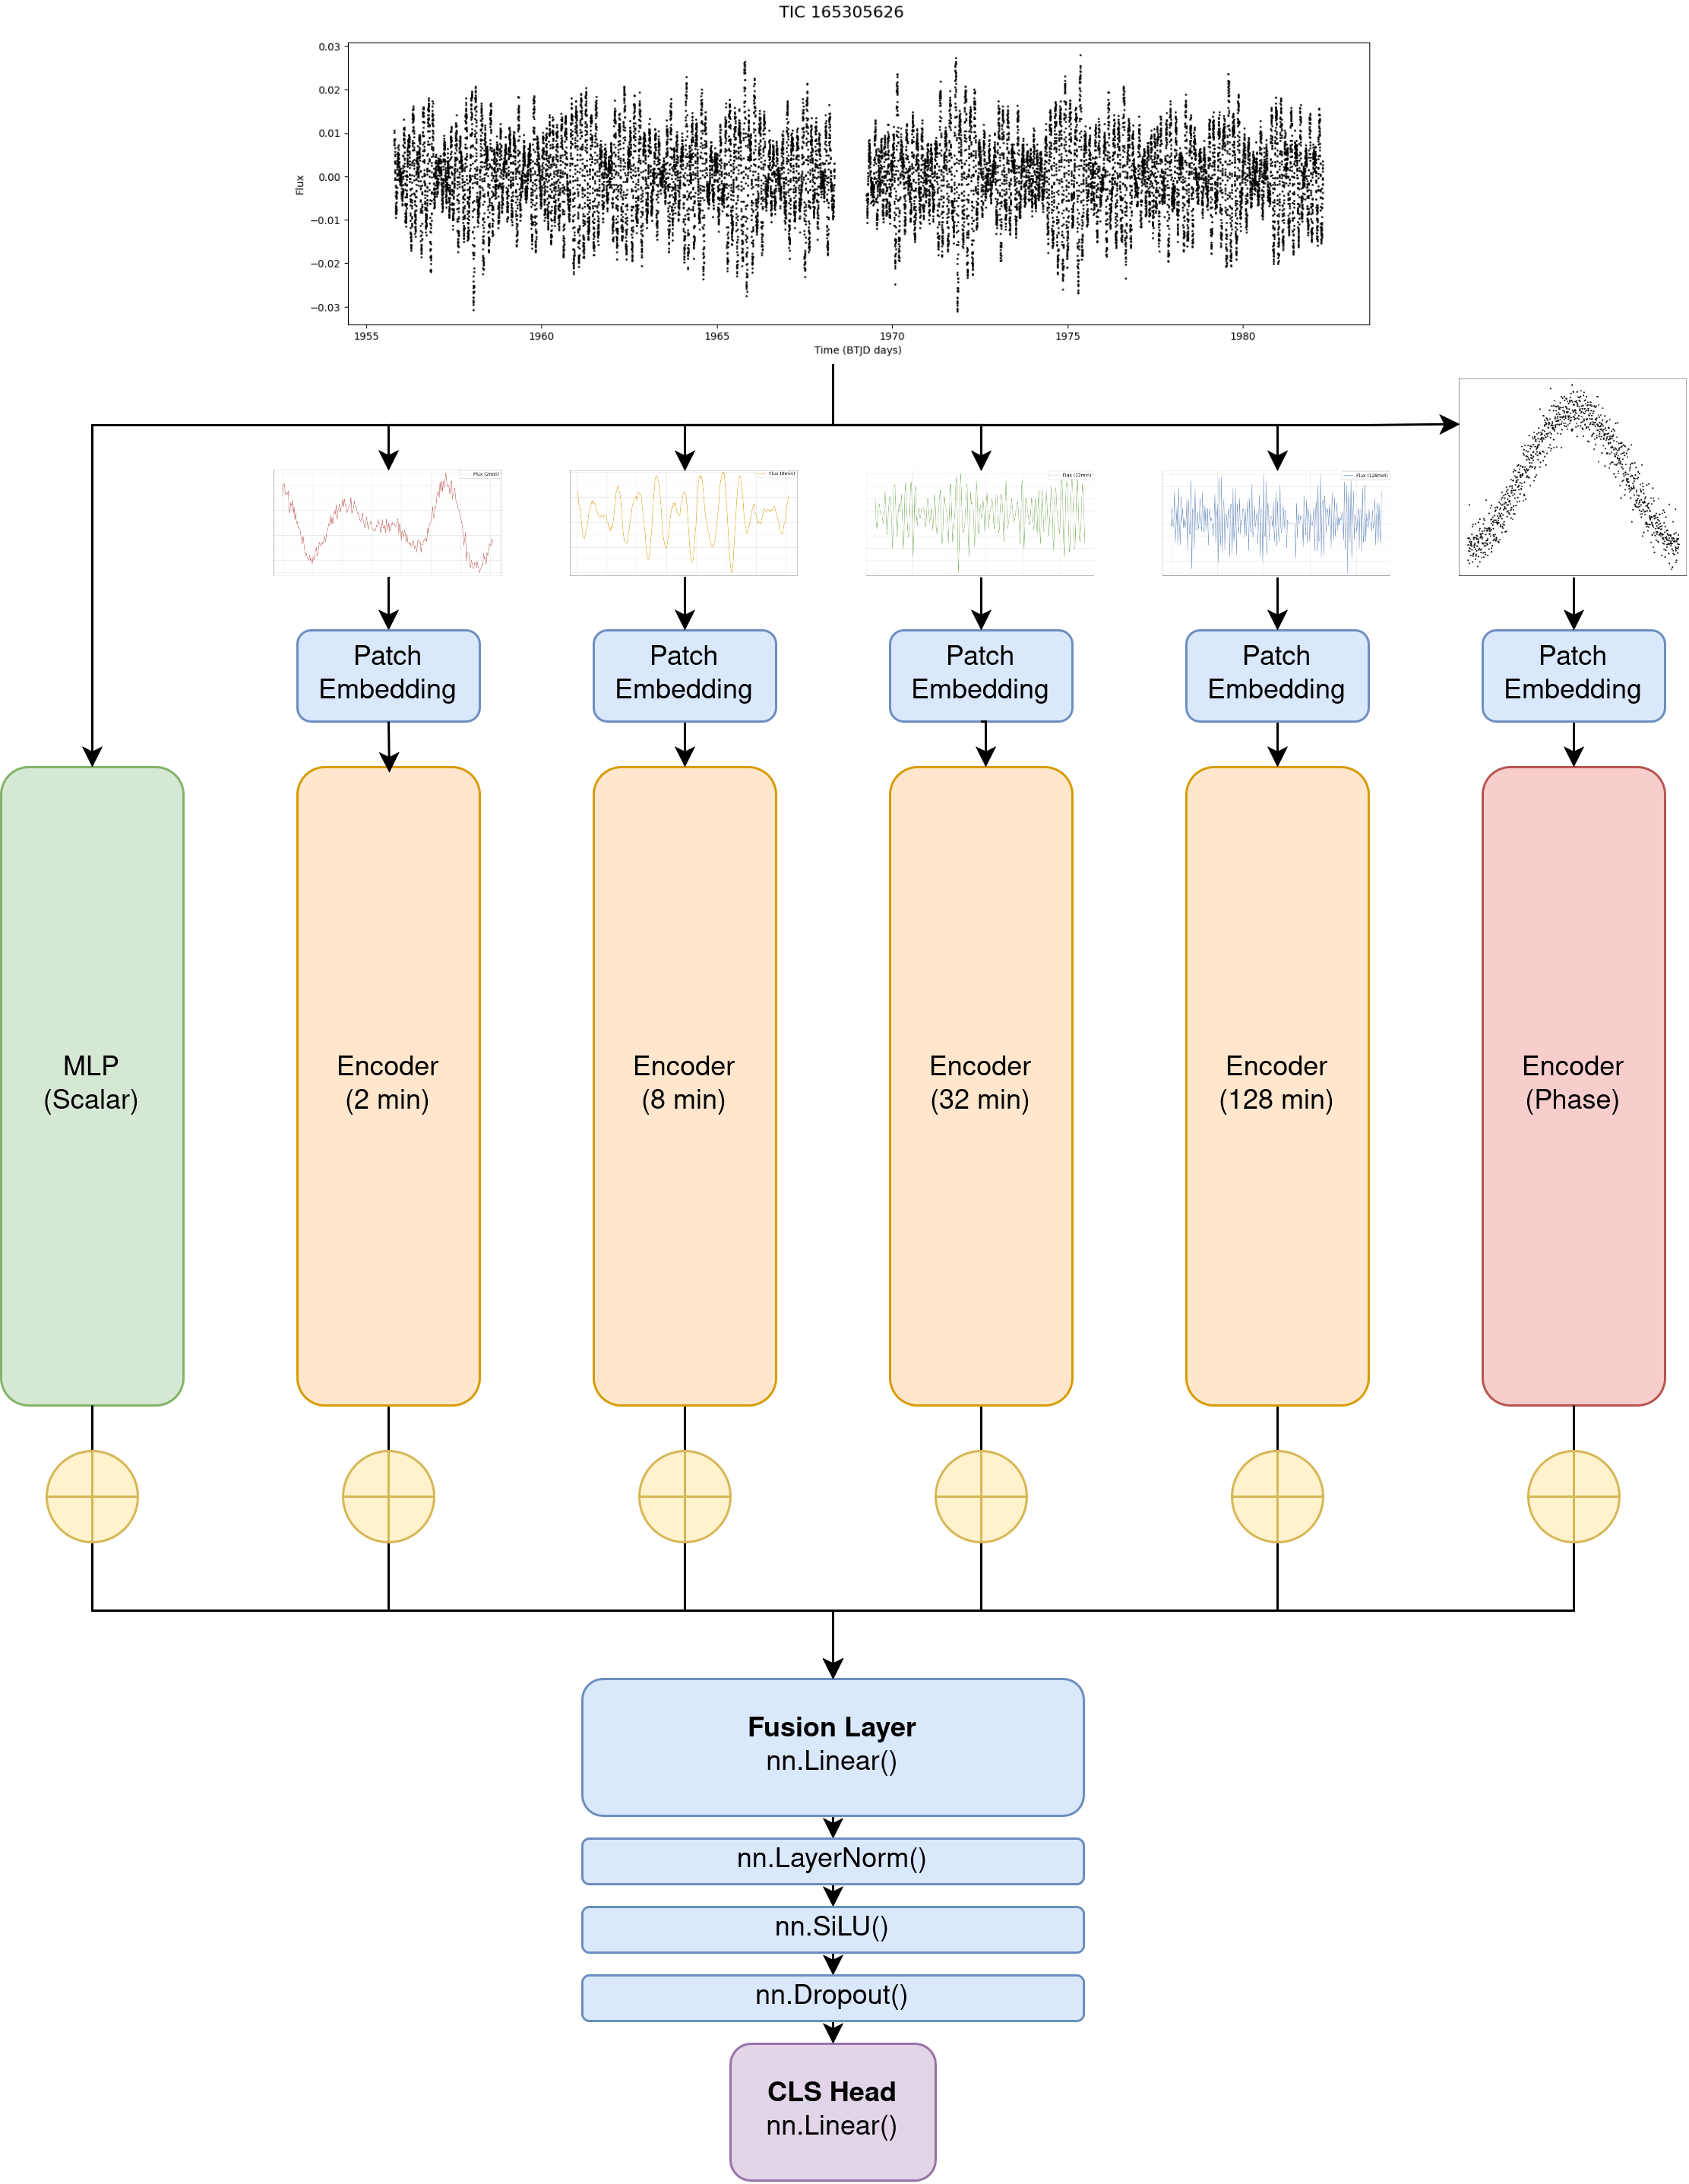
\includegraphics[width=\linewidth]{images/06/model_architecture}
    \caption[Model Architecture]{Proposed Model Architecture, each of the branches can be turned on/off separately, allowing arbitrary combinations of channels.}
    \label{fig:06_model_architecture}
\end{figure}

\FloatBarrier

\subsection{Embeddings}

We have experimented with two main types of embeddings:

\begin{itemize}
    \item \textbf{Learnable Embeddings.} While trivial to implement, they were prone to overfitting and didn't generalize as well.
    Another downside was the attention cost, since each data point turns into one token.
    \item \textbf{Patch Embeddings.} Similarly to \hyperref[subsec:04-base-transformer]{4.4.2 Base Transformer}, patch embeddings also performed really well on this task and were therefore used for most of the models.
\end{itemize}

\subsubsection{Statistical Patch Embeddings}

While even patch embeddings of raw flux values performed decently, we improved them by adding additional information computed from the patch.

For an input tensor of shape

\[
    (L, D)
\]

where $L$ is the sequence length and $D$ is the number of input channels ($\Phi$ and $\Phi_{\mathrm{err}}$), the tensor is reshaped into shape

\[
    (N, P, D)
\]

where $P$ is the selected patch size and $N = L / P$ is the number of resulting patches, to ensure divisibility by $P$, the sequence is padded as necessary.

For each patch, summary statistics are then computed, independently for each channel and using only valid positions according to the provided \hyperref[subsec:05-observation-gaps]{mask} to prevent invalid positions from influencing the result.

Specifically, the following features are computed for each patch $j$ and input channel $d$:

\begin{table}[H]
    \centering
    \small
    \renewcommand{\arraystretch}{1.3}
    \begin{tabularx}{\textwidth}{X c}
        \toprule
        \textbf{Parameter} & \textbf{Description} \tabularnewline
        \midrule
        $\mu_{j,d}$ & Mean \tabularnewline
        $\sigma_{j,d}$ & Standard Deviation \tabularnewline
        $\min_{j,d}$ & Minimum \tabularnewline
        $\max_{j,d}$ & Maximum \tabularnewline
        $m_{j,d}$ & Slope - approximated as $\frac{\mathrm{cov(input,time)}}{\mathrm{var(time)}}$ \tabularnewline
        $v$ & Fraction of valid points \tabularnewline
        \bottomrule
    \end{tabularx}
    \caption[Patch Statical Features]{Patch Statical Features}
    \label{tab:06_patch_statistical_featues}
\end{table}

The statistical features are then reshaped into vector of length $5D + 1$ (1~represents the valid point fraction), this vector is then projected into $d_{\mathrm{model}}$ using a compact 2 layer MLP.

The usage of statistical patch embeddings significantly improved the model performance by approximately $0.05 - 0.1 \Delta$ Macro F1.


\section{Implementation}

The implementation was again done in Python, with \textbf{PyTorch} and \textbf{Transformers} being the main libraries.
While initial prototyping was done using Jupyter notebooks, we decided to design and implement a modular framework that allows seamless running of different model configurations using only config files and minimal changes to the code.

\subsection{Structure}

The framework was developed as a self-contained python package:

\dirtree{%
    .1 /.
    .2 README.md \DTcomment{README file with documentation}.
    .2 \_\_main\_\_.py \DTcomment{Driver code}.
    .2 config.py \DTcomment{Experiment configuration}.
    .2 data.py \DTcomment{Dataset handling}.
    .2 evaluation.py \DTcomment{Metric computation}.
    .2 experiment.py \DTcomment{Experiment run orchestration}.
    .2 model.py \DTcomment{Implementation of the model components}.
    .2 trainer.py \DTcomment{Training run orchestration}.
    .2 utils.py \DTcomment{Utility and helper functions}.
}

\bigskip

The framework allows the user to setup the entire model configuration and training hyperparameters through a JSON configuration file.
Documentation and replicability of experiments if then trivial, since the original configuration file is saved alongside the results.
The framework also supports running multiple experiments sequentially in one run -- the driver code is only provided with a location of a directory that contains multiple configuration files and one experiment is then conducted for each of them.

Additionally, the trainer can continuously report the training progress to a Weights \& Biases\footnote{https://wandb.ai/} dashboard thas is accessible from the internet, allowing the user to remotely monitor long-running experiments.

\subsection{Saving Models}

Saving each model checkpoint quickly becomes memory intensive due to their large size, especially in the case of fine-tuned pretrained models.
To mitigate this issue, only one checkpoint was stored for each experiment.
This checkpoint was tracked by a custom callback triggered after each validation stage, TIC-level Macro F1 was computed and the tracked model was updated if improvement happened.

\subsection{Supported Transformer Architectures}

The framework allows configuration of the transformer architecture that is used in the transformer branches, the following architectures are supported

\begin{table}[H]
    \centering
    \footnotesize
    \renewcommand{\arraystretch}{1.3}
    \begin{tabularx}{\textwidth}{l c X}
        \toprule
        \textbf{Architecture} & \textbf{Type} & \textbf{Note} \tabularnewline
        \midrule
        Transformer & Transformer & The model is fully trained from scratch. \tabularnewline
        Chronos-2 & Pretrained TSFM\footnote{Time Series Foundation Model} & Accepts only raw flux values, handles tokenization and patching internally.  \tabularnewline
        Qwen 2.5 0.5B & Pretrained LLM & Largest model at around 1GB.   \tabularnewline
        \bottomrule
    \end{tabularx}
    \caption[Supported Transformer Architectures]{Supported Transformer Architectures}
    \label{tab:06_supported_transformer_architecture}
\end{table}

\subsubsection{Chronos-2}\label{subsubsec:06-chronos}

Chronos-2 is a 120M-parameter, encoder-only time series foundation model developed by Amazon.
While originally trained for time series forecasting, it can be fine-tuned for the classification task. \parencite{Ansari2025}


\section{Phase 1 -- Exploring Configurations}

In the first phase of experiments, various configurations of hyperparameters were tried to find a suitable baseline for further experiments.

\subsection{Patch Size}

\textbf{Patch Size} was one of the most influential parameters, multiple sizes from $4$ to $64$ were evaluated and $16$ was chosen as the best performing size.
Much larger and smaller values than $16$ performed significantly worse and either led to overfitting or did not converge reliably.

\subsection{Transformer Configuration}

The parameters for transformer configuration are intertwined with each other (for example, most publications recommend $d_{\mathrm{ff}} = 4 \cdot d_{\mathrm{model}}$).
Additionally, our experiments have shown that these parameters usually have some kind of \textbf{minimal viable value} -- models with lower values than the minimal viable value don't converge, however increasing it doesn't yield any further improvements.

The values that generally worked well for most configurations were:

\begin{table}[H]
    \centering
    \small
    \renewcommand{\arraystretch}{1.1}
    \begin{tabularx}{\textwidth}{X c}
        \toprule
        \textbf{Parameter} & \textbf{Value} \tabularnewline
        \midrule
        $n_{\mathrm{head}}$ & 8 \tabularnewline
        $n_{\mathrm{layers}}$ & 4 \tabularnewline
        $d_{\mathrm{model}}$ & 256 \tabularnewline
        $d_{\mathrm{ff}}$ & 1024 \tabularnewline
        $d_{\mathrm{fusion}}$ & 256 \tabularnewline
        \bottomrule
    \end{tabularx}
    \caption[Transformer Hyperparameters]{Transformer Hyperparameters}
    \label{tab:06_transformer_hyperparameters}
\end{table}

\subsection{Training}

Mutliple parameters for training were also explored:

\begin{itemize}
    \item \textbf{Learning Rate.} $5 \times 10^{-5}$ was chosen as a good baseline, since it achieved reliable convergence across most configurations.
    \item \textbf{Optimizer.} AdamW was chosen because it outperformed the simpler Adam optimizer.
    \item \textbf{Batch Size.} $64$ was at the upper limit of what could fit into the GPU VRAM, it also generally achieved slightly better validation performance than lower values.
    \item \textbf{Epochs.} $50$ was identified as a baseline, since it allowed most models to converge and show signs of overfitting at the end of the training.
    \item \textbf{Loss Function.} The proposed \hyperref[subsubsec:06-turbo-loss]{Segment \& Class Weighted Loss} was used.
\end{itemize}

\subsection{LR Scheduler}

Flat learning rate and multiple LR schedulers were tried, \textbf{CosineAnnealingLR} was then chosen due to its best performance.

The cosine annealing scheduler gradually decreases the learning rate $\eta$, following a cosine curve.

\[
    \eta_t = \eta_{\min} + \frac{1}{2}(\eta_{\max} - \eta_{\min})\left(1 + \cos\left(\pi \cdot \frac{t}{T_{\text{max}}}\right)\right)
\]

\begin{figure}[!htbp]
    \centering
    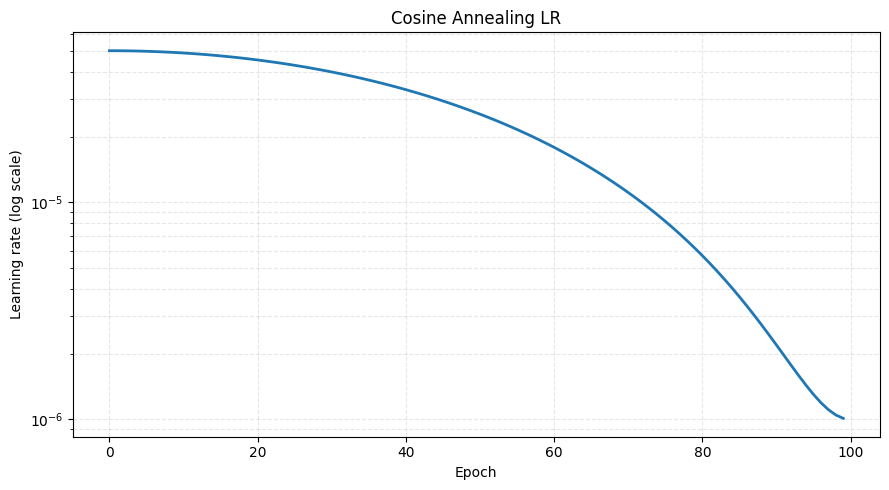
\includegraphics[width=0.6\linewidth]{images/06/cosine_annealing}
    \caption[Cosine Annealing LR]{Evolution of the learning rate, decreasing from $5 \times 10^{-5}$ to $1 \times 10^{-6}$}.
    \label{fig:06_cosine_annealing}
\end{figure}

\FloatBarrier

\subsection{Balanced Sampling}

This method was tried mainly on \textbf{Task B} due to the imbalanced dataset, however it limited the generalization of the model by over-predicting the eclipsing class.
It was therefore not used in future models.


\section{Phase 2 -- Basic Models}

Settings for a reasonably good baseline model were explored and identified in the previous phase.
In this phase, \textbf{12} experiments were conducted with a fixed set of hyperparameters, the only difference being the activated channels.

\begin{table}[H]
    \centering
    \small
    \renewcommand{\arraystretch}{1.1}
    \begin{tabularx}{\textwidth}{X c}
        \toprule
        \textbf{Parameter} & \textbf{Value} \tabularnewline
        \midrule
        Epochs & 50 \tabularnewline
        Learning Rate & 5 \times $10^{-5}$ \tabularnewline
        Batch Size & 64 \tabularnewline
        $n_{\mathrm{head}}$ & 8 \tabularnewline
        $n_{\mathrm{layers}}$ & 4 \tabularnewline
        $d_{\mathrm{model}}$ & 256 \tabularnewline
        $d_{\mathrm{ff}}$ & 1024 \tabularnewline
        $d_{\mathrm{fusion}}$ & 256 \tabularnewline
        Patch Size & 16 \tabularnewline
        Dropout & 0.15 \tabularnewline
        Loss & WeightedLoss \tabularnewline
        Optimizer & AdamW \tabularnewline
        Weight Decay & 1 \times $10^{-2}$ \tabularnewline
        \bottomrule
    \end{tabularx}
    \caption[Phase 2 Hyperparameters]{Phase 2 Hyperparameters}
    \label{tab:06_phase_2_hyperparameters}
\end{table}

\subsection{1-Channel Transformers}

Initially, only $1$ of the $4$ available flux sequence channels was selected at a time.

\subsubsection{Task A}

The training took around $20$ minutes for each of the models.

\begin{table}[H]
    \centering
    \small
    \renewcommand{\arraystretch}{1.1}
    \begin{tabularx}{\textwidth}{X c c c c}
        \toprule
        \textbf{Channel} & \textbf{Accuracy} & \textbf{Macro F1} & \textbf{TIC Accuracy} & \textbf{TIC Macro F1}  \tabularnewline
        \midrule
        2-min & 0.72 & 0.72 & 0.84 & 0.84 \tabularnewline
        8-min & 0.78 & 0.78 & 0.87 & 0.87 \tabularnewline
        32-min & 0.80 & 0.80 & 0.87 & 0.87 \tabularnewline
        128-min & 0.77 & 0.77 & 0.84 & 0.84 \tabularnewline
        \bottomrule
    \end{tabularx}
    \caption[Phase 2 -- 1-Channel Transformer Metrics (A)]{1-Channel Transformer Validation Metrics (Task A)}
    \label{tab:06_phase_2_1_channel_a}
\end{table}

\FloatBarrier

The 32-min channel performed the best, it was therefore selected for further evaluation.

\begin{figure}[!htbp]
    \centering
    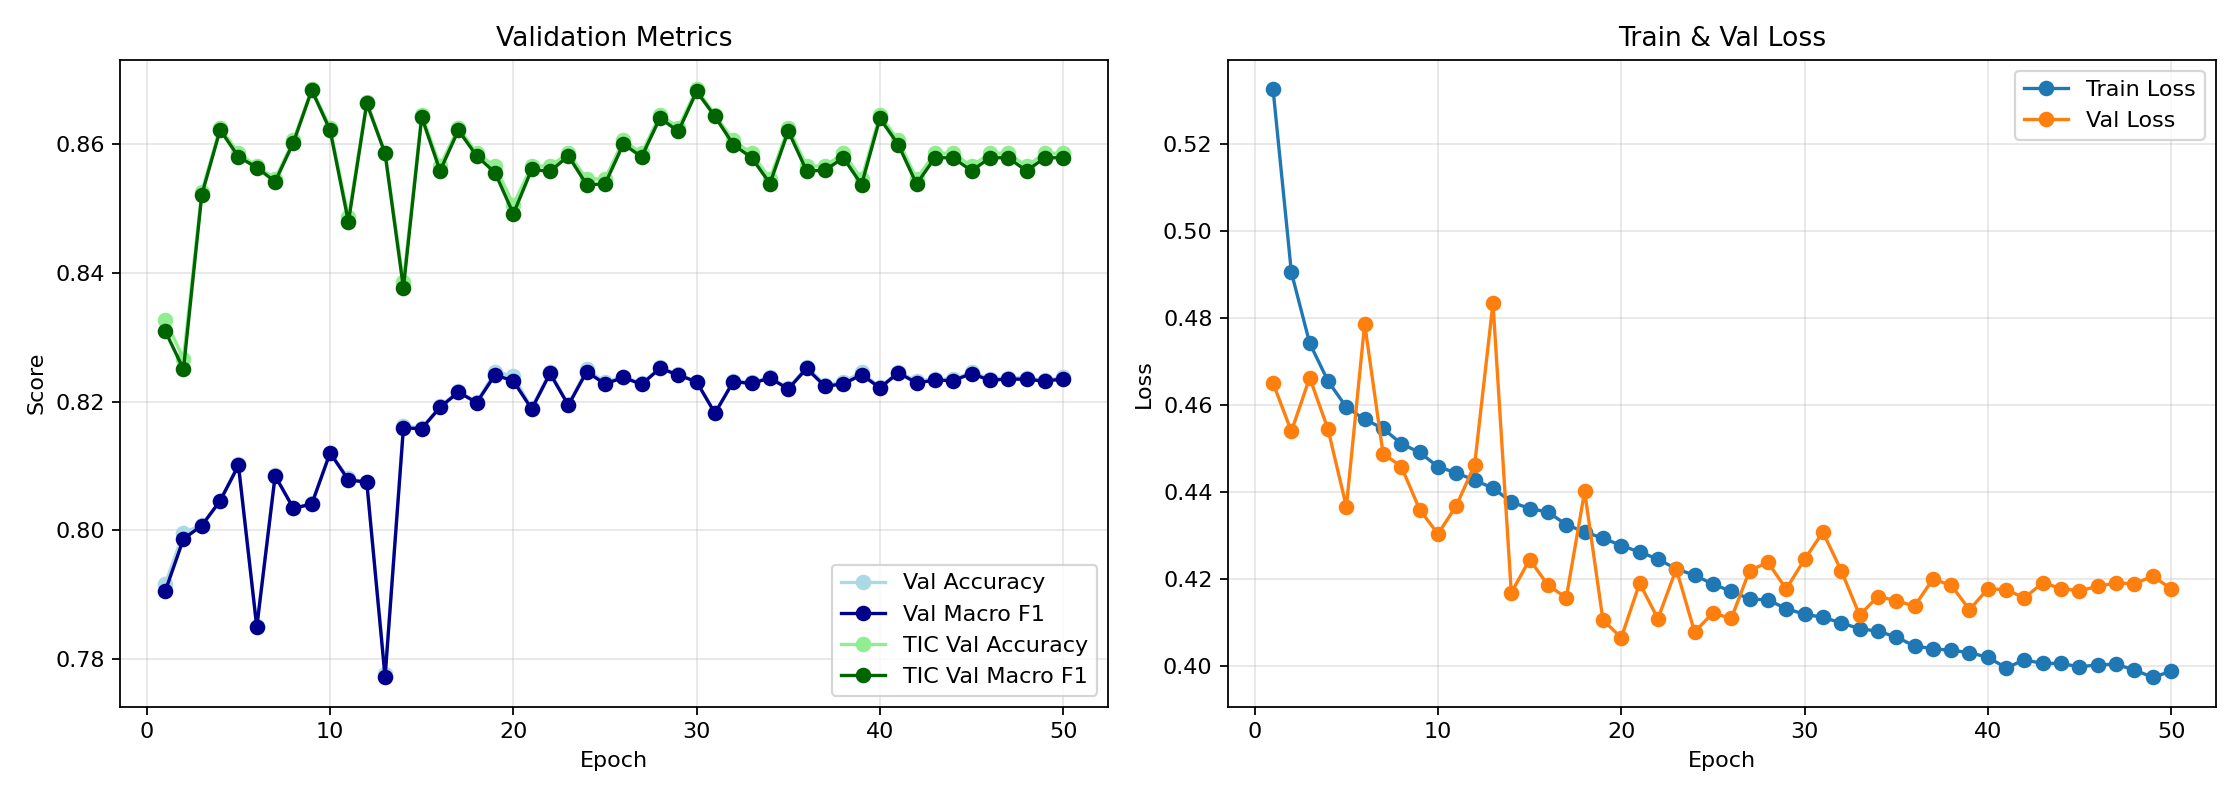
\includegraphics[width=\linewidth]{images/06/phase2_A_1c_training_curves}
    \caption[Phase 2 -- 32-min Channel Transformer Training Curves (A)]{32-min Channel Transformer Training Curves (Task A)}
    \label{fig:06_phase_2_32_min_channel_transformer_training_curves_a}
\end{figure}

\FloatBarrier

The training loss steadily continued to decrease throughout the training, the validation loss also decrease until around epoch $25$, although it was much more unstable.
After epoch $25$, the model probably started overfitting.

It should be noted the disparity between segment-level and TIC-level metrics ($\Delta \approx 0.04$) throughout the entire training, the segment logit aggregation seems to work really well for blabel prediction of individual stars.

\begin{table}[H]
    \centering
    \footnotesize
    \renewcommand{\arraystretch}{1.1}

    \begin{minipage}[t]{0.32\textwidth}
        \centering
        \begin{tabularx}{\textwidth}{X c}
            \toprule
            \textbf{Metric} & \textbf{Score} \tabularnewline
            \midrule
            Accuracy    &  0.8041 \tabularnewline
            Macro F1    & 0.8041 \tabularnewline
            TIC Accuracy & 0.8685 \tabularnewline
            TIC Macro F1 & 0.8636 \tabularnewline
            \bottomrule
        \end{tabularx}
    \end{minipage}
    \hfill
    \begin{minipage}[t]{0.64\textwidth}
        \centering
        \footnotesize
        \begin{tabularx}{\textwidth}{X c c c c c}
            \toprule
            \textbf{Class} & \textbf{Precision} & \textbf{Recall} & \textbf{F1-score} & \textbf{Support} \tabularnewline
            \midrule
            N & 0.87 & 0.88 & 0.87 & 259 \tabularnewline
            V & 0.87 & 0.86 & 0.86 & 243   \tabularnewline
            \bottomrule
        \end{tabularx}
    \end{minipage}

    \caption[Phase 2 -- 32-min Transformer Validation Metrics (A)]{Validation Metrics (Task A)}
    \label{tab:06_phase_2_32_min_channel_transformer_validation_,etrics_a}
\end{table}

\FloatBarrier

The validation predictions for both classes were balanced, none of them was visibly preferred.

\subsubsection{Task B}

The training took around $5$ minutes for each of the models, which is proportional to the difference of sizes between the two datasets.

\begin{table}[H]
    \centering
    \small
    \renewcommand{\arraystretch}{1.1}
    \begin{tabularx}{\textwidth}{X c c c c}
        \toprule
        \textbf{Channel} & \textbf{Accuracy} & \textbf{Macro F1} & \textbf{TIC Accuracy} & \textbf{TIC Macro F1}  \tabularnewline
        \midrule
        2-min & 0.66 & 0.59 & 0.72 & 0.69 \tabularnewline
        8-min & 0.77 & 0.72 & 0.86 & 0.82 \tabularnewline
        32-min & 0.83 & 0.81 & 0.87 & 0.86 \tabularnewline
        128-min & 0.88 & 0.88 & 0.90 & 0.91 \tabularnewline
        \bottomrule
    \end{tabularx}
    \caption[Phase 2 -- 1-Channel Transformer Metrics (B)]{1-Channel Transformer Validation Metrics (Task B)}
    \label{tab:06_phase_2_1_channel_b}
\end{table}

\FloatBarrier

The 128-min channel performed the best, it was therefore chosen for further evaluation.

\begin{figure}[!htbp]
    \centering
    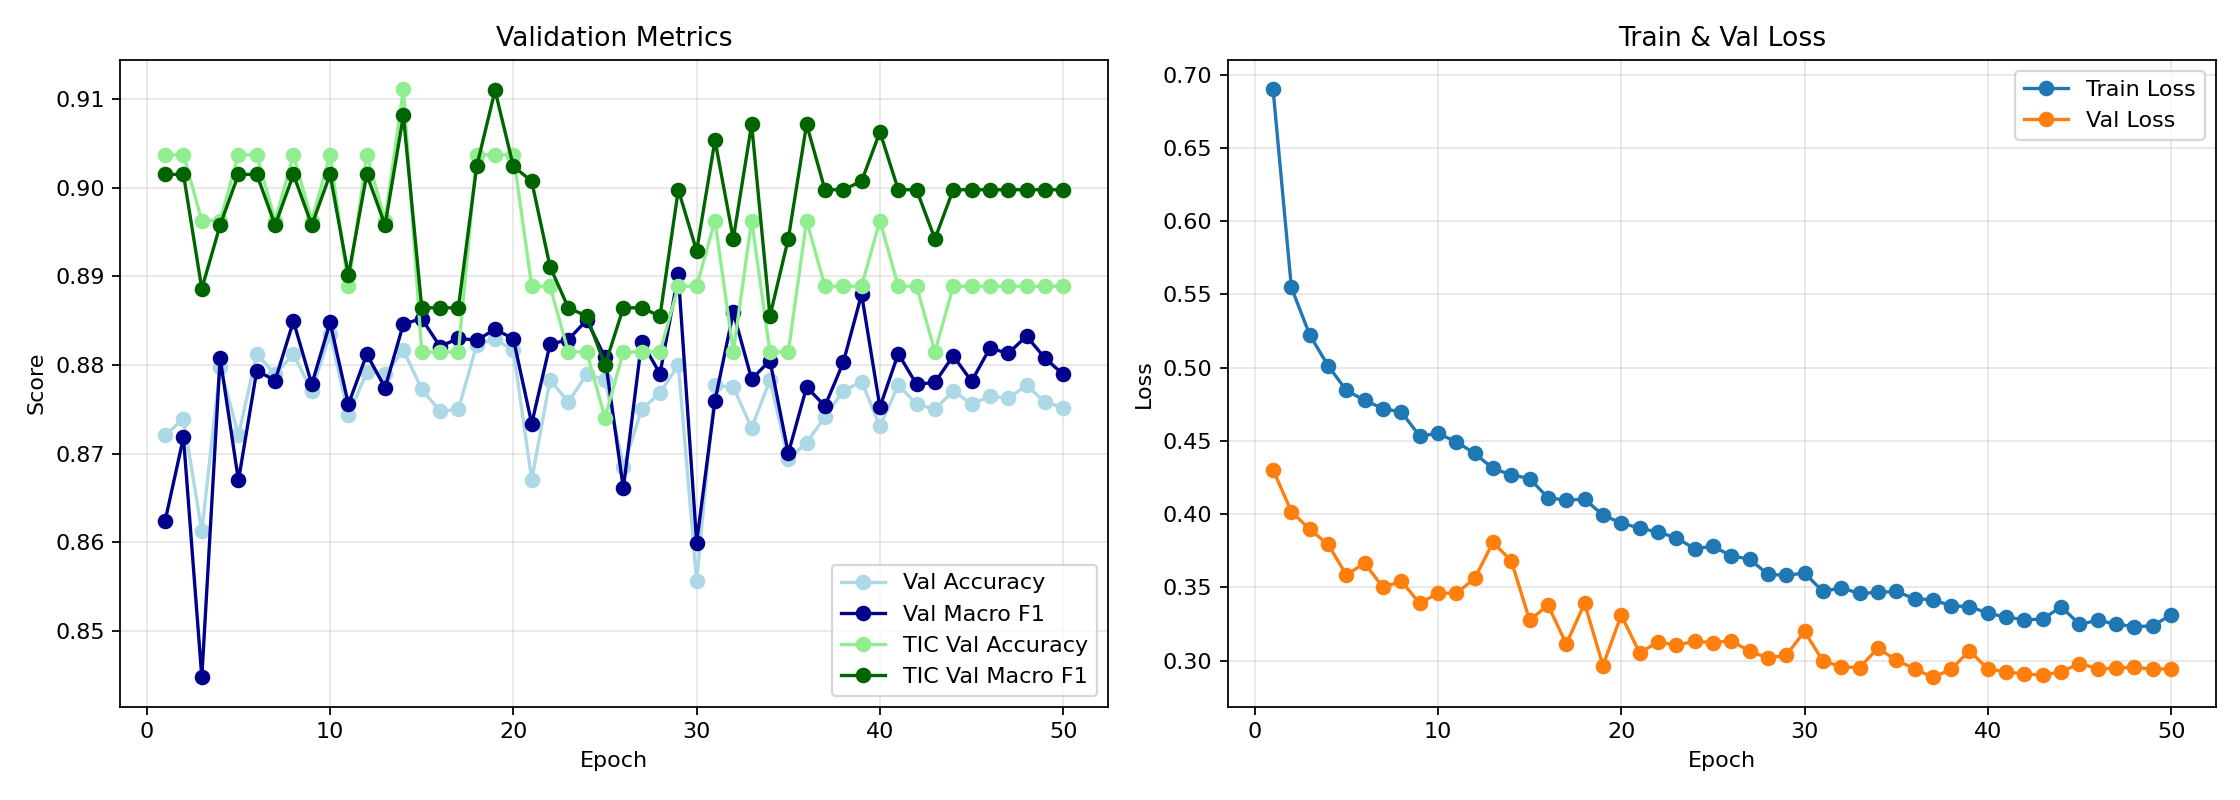
\includegraphics[width=\linewidth]{images/06/phase2_B_1c_training_curves}
    \caption[Phase 2 -- 128-min Channel Transformer Training Curves (B)]{128-min Channel Transformer Training Curves (Task B)}
    \label{fig:06_phase_2_128_min_channel_transformer_training_curves_b}
\end{figure}

\FloatBarrier

While the training loss continued to decrease, the validation loss went down and stagnated at around $0.3$.
The model was probably too simple to overfit and would've benefitted from more parameters.

The TIC-level aggregated predictions were again significantly better than raw segment-level predictions.

\begin{table}[H]
    \centering
    \footnotesize
    \renewcommand{\arraystretch}{1.1}

    \begin{minipage}[t]{0.32\textwidth}
        \centering
        \begin{tabularx}{\textwidth}{X c}
            \toprule
            \textbf{Metric} & \textbf{Score} \tabularnewline
            \midrule
            Accuracy    &  0.8829 \tabularnewline
            Macro F1    & 0.8840 \tabularnewline
            TIC Accuracy & 0.9037 \tabularnewline
            TIC Macro F1 & 0.9110 \tabularnewline
            \bottomrule
        \end{tabularx}
    \end{minipage}
    \hfill
    \begin{minipage}[t]{0.64\textwidth}
        \centering
        \footnotesize
        \begin{tabularx}{\textwidth}{X c c c c c}
            \toprule
            \textbf{Class} & \textbf{Precision} & \textbf{Recall} & \textbf{F1-score} & \textbf{Support} \tabularnewline
            \midrule
            E & 1.00 & 0.93 & 0.97 & 15 \tabularnewline
            P & 0.95 & 0.90 & 0.92 & 81   \tabularnewline
            R & 0.80 & 0.90 & 0.84 & 39 \tabularnewline
            \bottomrule
        \end{tabularx}
    \end{minipage}

    \caption[Phase 2 -- 128-min Transformer Validation Metrics (B)]{Validation Metrics (Task B)}
    \label{tab:06_phase_2_128_min_channel_transformer_validation_,etrics_b}
\end{table}

The model performed really well on the \textbf{eclipsing} class, which may seem surprising, because it's the class with the lowest sample count.
However, the light curves of eclipsing stars are the most recognizable with sharp peaks that are strongly periodic.
Although it good also be caused by random chance, since even one additional (un)successful classification can heavily skew the Macro F1 score.

\subsection{Multi-Channel Transformers}

After the single-channel baseline models, two additional configurations were evaluated - one with all 6 channels\footnote{Only 5 of those channels utilize the transformer architecture -- the 6th channel consists of scalar features that are handled by a non-transformer MLP.} enabled and one with only the 4 flux channels enabled (no phase-folded information).

The training took around $50$ minutes for the smaller model and around $70$ for the larger one on Task A and was proportionally shorter on Task B\@.

\subsubsection{Task A}

\begin{table}[H]
    \centering
    \small
    \renewcommand{\arraystretch}{1.1}
    \begin{tabularx}{\textwidth}{X c c c c}
        \toprule
        \textbf{Configuration} & \textbf{Accuracy} & \textbf{Macro F1} & \textbf{TIC Accuracy} & \textbf{TIC Macro F1}  \tabularnewline
        \midrule
        4-channel & 0.85 & 0.85 & 0.90 & 0.90 \tabularnewline
        6-channel & 0.88 & 0.88 & 0.91 & 0.91 \tabularnewline
        \bottomrule
    \end{tabularx}
    \caption[Phase 2 -- Multi-Channel Transformer Metrics (A)]{Multi-Channel Transformer Validation Metrics (Task A)}
    \label{tab:06_phase_2_multi_channel_a}
\end{table}

\FloatBarrier

The 6-channel model performed better, it was therefore selected for further evaluation.

\begin{figure}[!htbp]
    \centering
    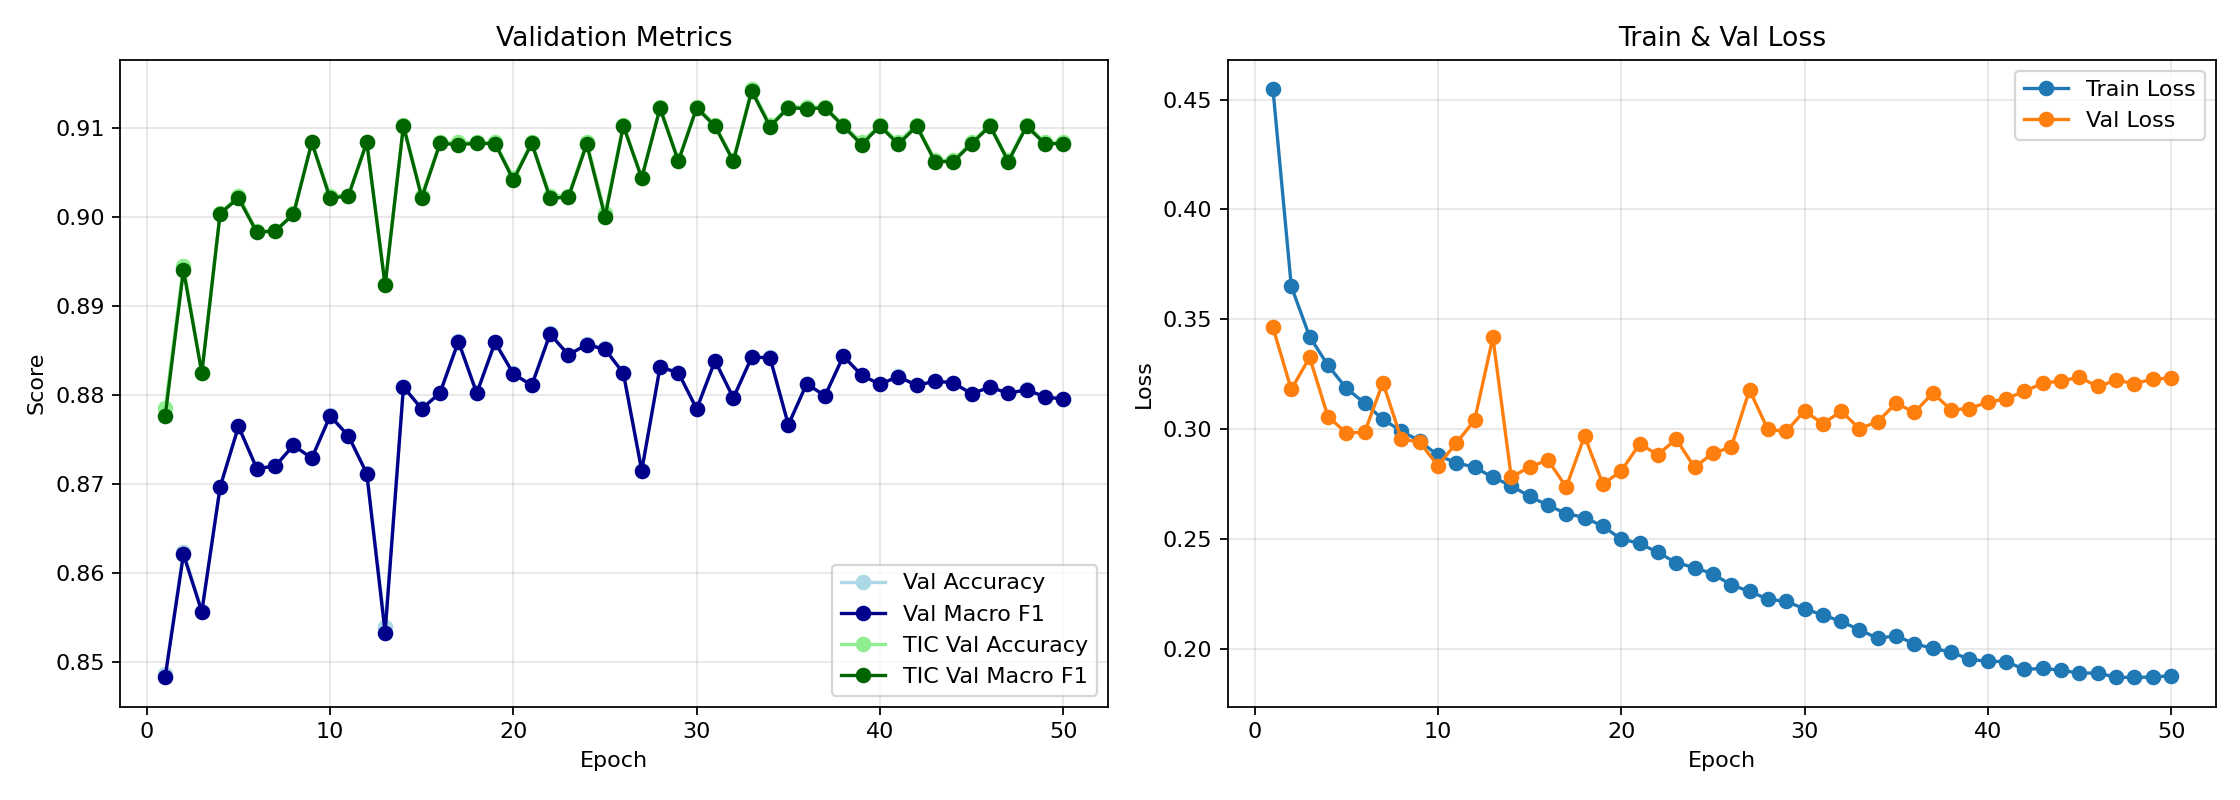
\includegraphics[width=\linewidth]{images/06/phase2_A_6c_training_curves}
    \caption[Phase 2 -- 6-Channel Transformer Training Curves (A)]{6-Channel Transformer Training Curves (Task A)}
    \label{fig:06_phase_2_6_channel_transformer_training_curves_a}
\end{figure}

\FloatBarrier

The training loss continued to decrease and diverged from the validation loss at around epoch $20$, TIC-level Macro F1 stagnated while segment-level Macro F1 continued to decrease as the model probably overfitted.

\begin{table}[H]
    \centering
    \footnotesize
    \renewcommand{\arraystretch}{1.1}

    \begin{minipage}[t]{0.32\textwidth}
        \centering
        \begin{tabularx}{\textwidth}{X c}
            \toprule
            \textbf{Metric} & \textbf{Score} \tabularnewline
            \midrule
            Accuracy    &  0.8527 \tabularnewline
            Macro F1    & 0.8527 \tabularnewline
            TIC Accuracy & 0.8984 \tabularnewline
            TIC Macro F1 & 0.8983 \tabularnewline
            \bottomrule
        \end{tabularx}
    \end{minipage}
    \hfill
    \begin{minipage}[t]{0.64\textwidth}
        \centering
        \footnotesize
        \begin{tabularx}{\textwidth}{X c c c c c}
            \toprule
            \textbf{Class} & \textbf{Precision} & \textbf{Recall} & \textbf{F1-score} & \textbf{Support} \tabularnewline
            \midrule
            N & 0.91 & 0.90 & 0.90 & 259 \tabularnewline
            V & 0.89 & 0.90 & 0.90 & 243   \tabularnewline
            \bottomrule
        \end{tabularx}
    \end{minipage}

    \caption[Phase 2 -- 6-Channel Transformer Validation Metrics (A)]{Validation Metrics (Task A)}
    \label{tab:06_phase_2_6_channel_transformer_validation_,etrics_a}
\end{table}

\FloatBarrier

The validation predictions for both classes were again balanced.

\subsubsection{Task B}

\begin{table}[H]
    \centering
    \small
    \renewcommand{\arraystretch}{1.1}
    \begin{tabularx}{\textwidth}{X c c c c}
        \toprule
        \textbf{Configuration} & \textbf{Accuracy} & \textbf{Macro F1} & \textbf{TIC Accuracy} & \textbf{TIC Macro F1}  \tabularnewline
        \midrule
        4-channel & 0.87 & 0.88 & 0.92 & 0.92 \tabularnewline
        6-channel & 0.89 & 0.89 & 0.92 & 0.92 \tabularnewline
        \bottomrule
    \end{tabularx}
    \caption[Phase 2 -- 1-Channel Transformer Metrics (B)]{1-Channel Transformer Validation Metrics (Task B)}
    \label{tab:06_phase_2_1_channel_bx}
\end{table}

\FloatBarrier

The 6-channel model again outperformed the 4-channel, although almost negligibly.

\begin{figure}[!htbp]
    \centering
    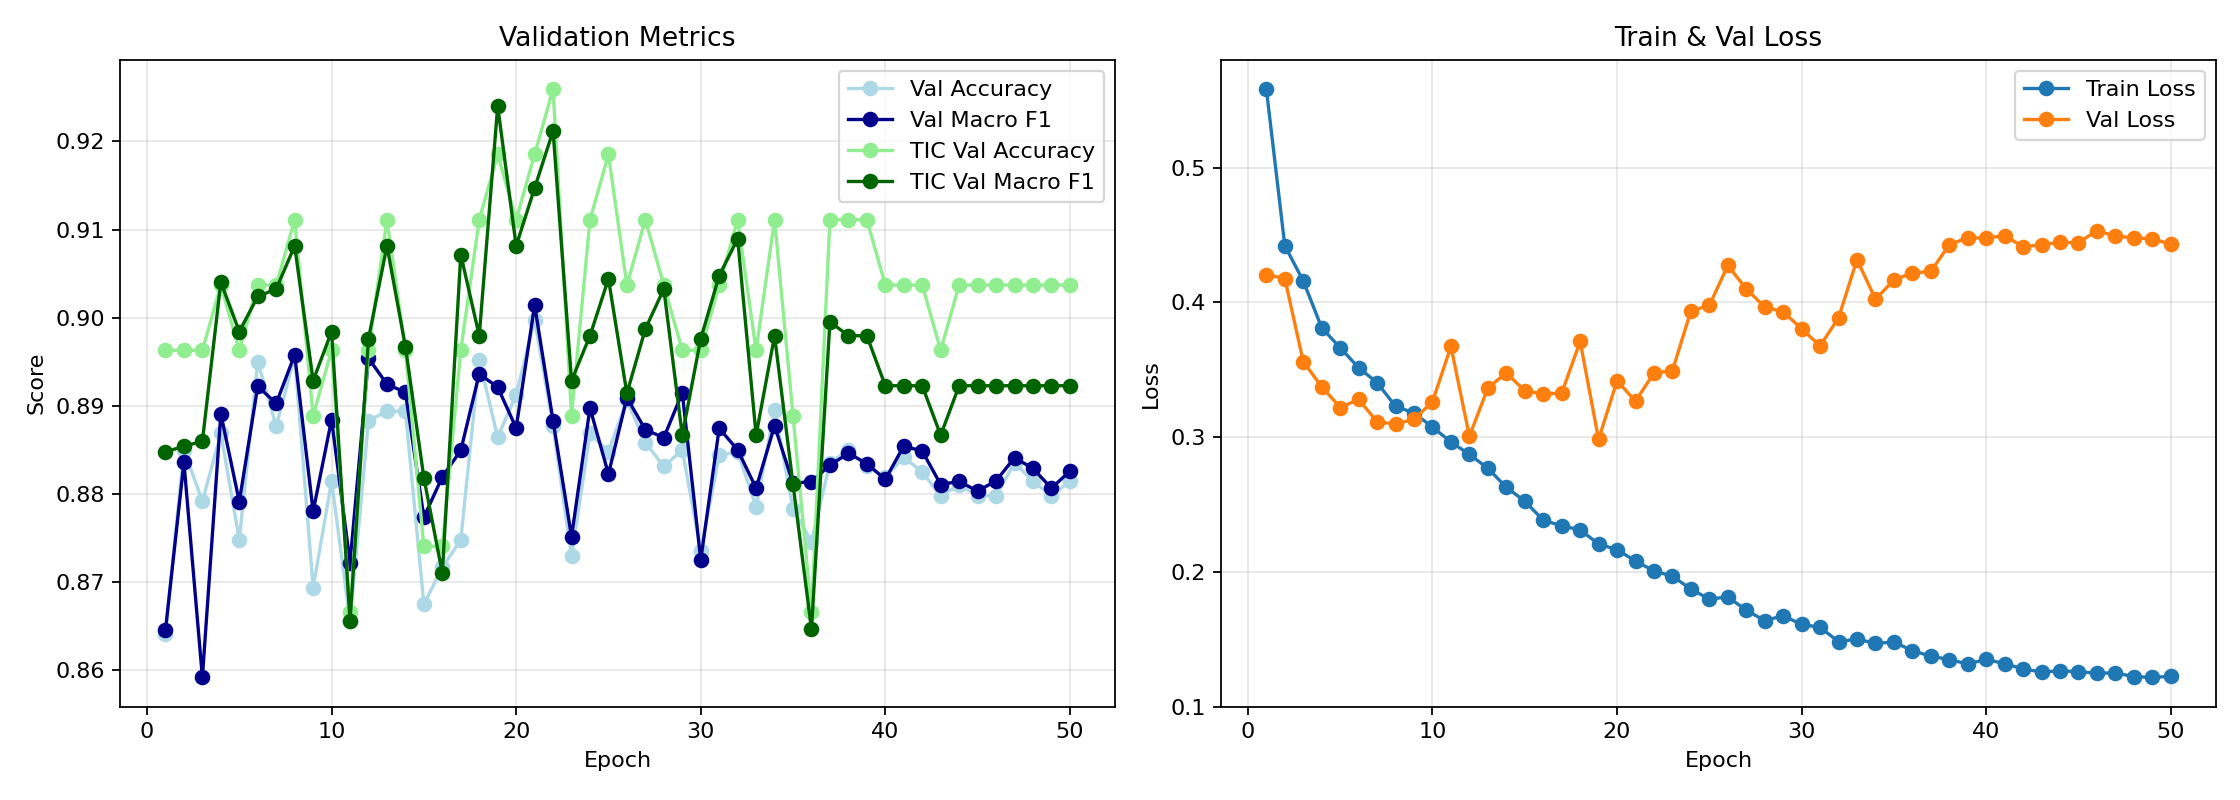
\includegraphics[width=\linewidth]{images/06/phase2_B_6c_training_curves}
    \caption[Phase 2 -- 6-Channel Transformer Training Curves (B)]{6-Channel Transformer Training Curves (Task B)}
    \label{fig:06_phase_2_6_channel_transformer_training_curves_b}
\end{figure}

\FloatBarrier

The training loss decreased steadily and diverged from the validation loss quite early, after epoch $10$, validation metrics showed unstable behavior throughout the whole training.

\begin{table}[H]
    \centering
    \footnotesize
    \renewcommand{\arraystretch}{1.1}

    \begin{minipage}[t]{0.32\textwidth}
        \centering
        \begin{tabularx}{\textwidth}{X c}
            \toprule
            \textbf{Metric} & \textbf{Score} \tabularnewline
            \midrule
            Accuracy    &  0.8867 \tabularnewline
            Macro F1    & 0.8921 \tabularnewline
            TIC Accuracy & 0.9185 \tabularnewline
            TIC Macro F1 & 0.9240 \tabularnewline
            \bottomrule
        \end{tabularx}
    \end{minipage}
    \hfill
    \begin{minipage}[t]{0.64\textwidth}
        \centering
        \footnotesize
        \begin{tabularx}{\textwidth}{X c c c c c}
            \toprule
            \textbf{Class} & \textbf{Precision} & \textbf{Recall} & \textbf{F1-score} & \textbf{Support} \tabularnewline
            \midrule
            E & 1.00 & 0.93 & 0.97 & 15 \tabularnewline
            P & 0.97 & 0.90 & 0.94 & 81   \tabularnewline
            R & 0.80 & 0.95 & 0.87 & 39 \tabularnewline
            \bottomrule
        \end{tabularx}
    \end{minipage}

    \caption[Phase 2 -- 6-Channel Transformer Validation Metrics (B)]{Validation Metrics (Task B)}
    \label{tab:06_phase_2_6_channel_transformer_validation_,etrics_b}
\end{table}

The model has shown great classification performance for all of the classes, however it may not be able to generalize well due to strong signs of overfitting from the training metrics.


\section{Phase 3 -- Pretrained Model Fine-Tuning}

In this phase, $2$ different pretrained models were fined-tuned:

\begin{itemize}
    \item \textbf{Chronos-2.} A 120M parameter pretrained TSFM, originally trained for time series forecasting.
    \item \textbf{Qwen 2.5 0.5B.} A 500M parameter pretrained LLM, designed for text completion.
\end{itemize}

We have decided to not utilize pretrained vision transformers in our experiments, mainly because we believe the task is fundamentally 1-dimensional at the physical level.

Both fine-tunes were performed with \hyperref[subsubsec:03-lora]{LoRA} (the original model weights remained frozen), the following parameters were used:

\begin{table}[H]
    \centering
    \small
    \renewcommand{\arraystretch}{1.1}
    \begin{tabularx}{\textwidth}{X c}
        \toprule
        \textbf{Parameter} & \textbf{Value} \tabularnewline
        \midrule
        Epochs & 10 \tabularnewline
        Learning Rate & 5 \times $10^{-5}$ \tabularnewline
        LoRA $r$ & 8 \tabularnewline
        LoRA $\alpha$ & 16 \tabularnewline
        Batch Size & 64 (32 for Qwen) \tabularnewline
        Patch Size & 16 (Chronos-2 expects the raw flux) \tabularnewline
        Dropout & 0.15 \tabularnewline
        Loss & WeightedLoss \tabularnewline
        Optimizer & AdamW \tabularnewline
        Weight Decay & 1 \times $10^{-2}$ \tabularnewline
        \bottomrule
    \end{tabularx}
    \caption[Phase 2 Hyperparameters]{Phase 2 Hyperparameters}
    \label{tab:06_phase_3_hyperparameters}
\end{table}

Both models were trained on all 6 available channels, batch size needed to be reduced for Qwen due to memory constraints.

The number of epochs was also reduced, because the fine-tuning of pretraining generally takes significantly less training steps compared to training from scratch.
However, because the pretrained models are much larger than the original transformers, the training can still take significant amounts of time.

\subsection{Chronos-2}

The training took around $100$ and $30$ minutes for tasks A and B respectively.

\subsubsection{Task A}

\begin{figure}[!htbp]
    \centering
    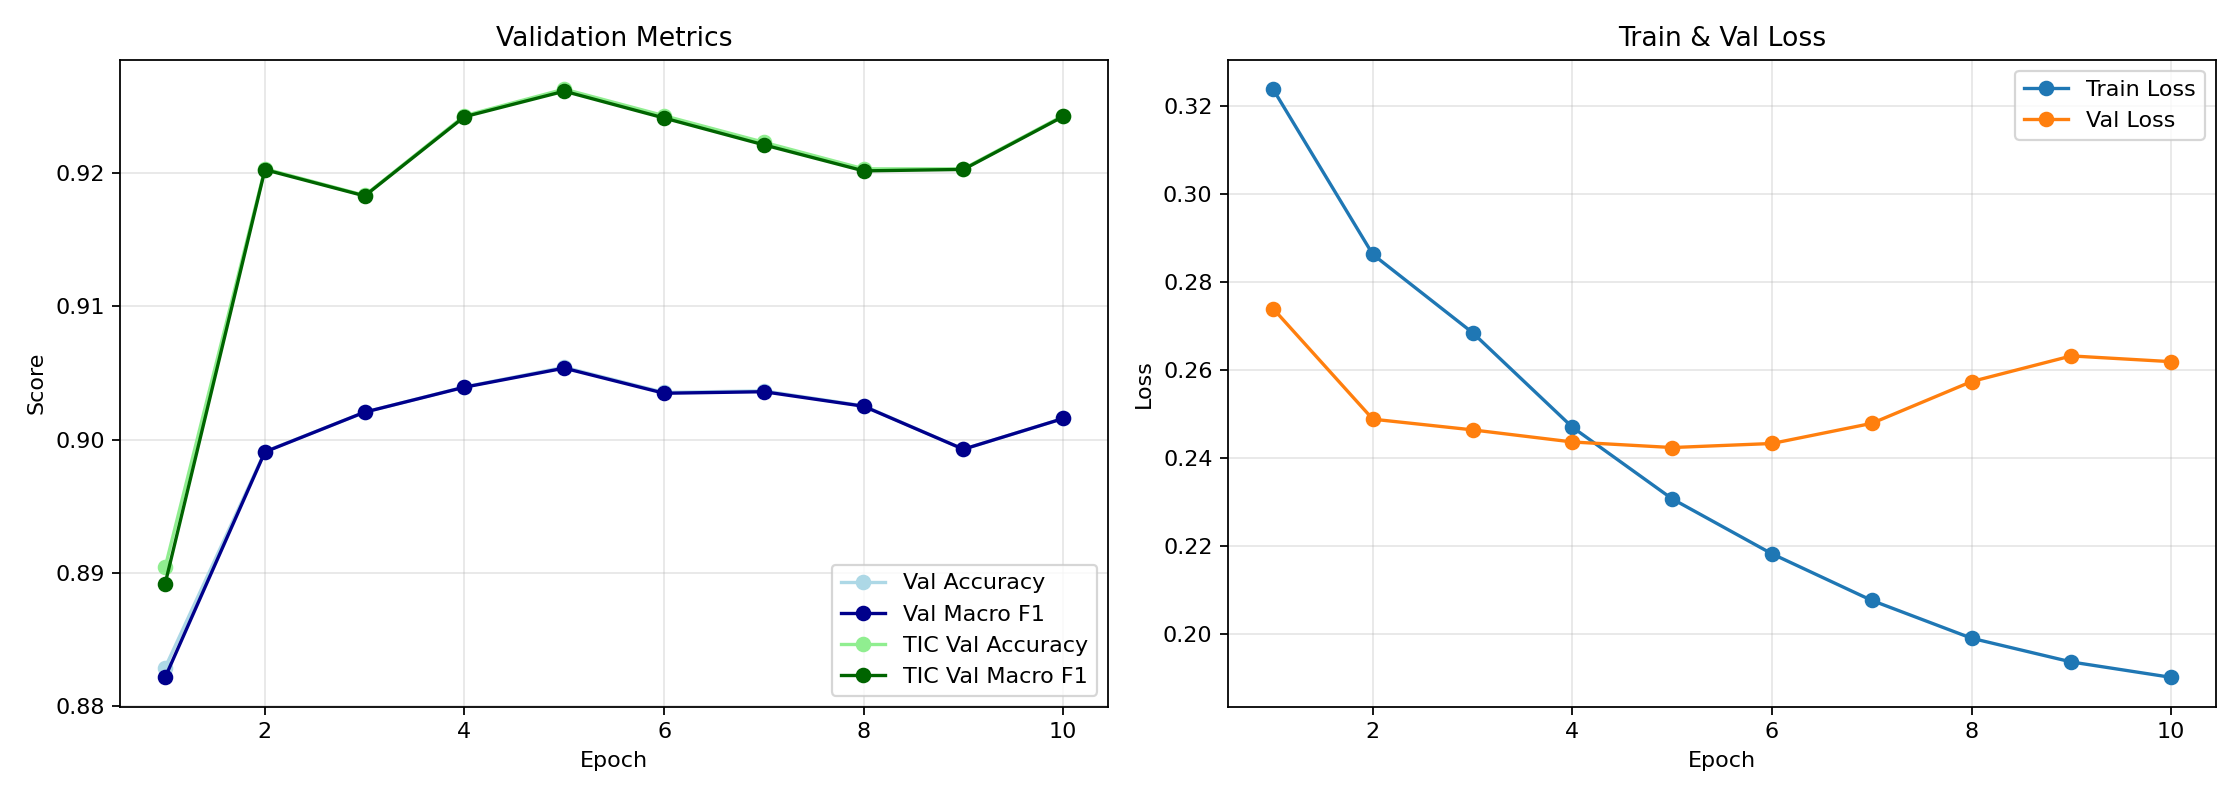
\includegraphics[width=\linewidth]{images/06/phase3_A_chronos_training_curves}
    \caption[Phase 3 -- Chronos-2 Training Curves (A)]{Chronos-2 Training Curves (Task A)}
    \label{fig:06_phase_3_chronos_training_curves_A}
\end{figure}

\FloatBarrier

The training loss steadily decreased and diverged from the validation loss at around epoch $4$, the best TIC Val Macro F1 was observed at epoch $5$.

\begin{table}[H]
    \centering
    \footnotesize
    \renewcommand{\arraystretch}{1.1}

    \begin{minipage}[t]{0.32\textwidth}
        \centering
        \begin{tabularx}{\textwidth}{X c}
            \toprule
            \textbf{Metric} & \textbf{Score} \tabularnewline
            \midrule
            Accuracy    &  0.9054 \tabularnewline
            Macro F1    & 0.9054 \tabularnewline
            TIC Accuracy & 0.9263 \tabularnewline
            TIC Macro F1 & 0.9261 \tabularnewline
            \bottomrule
        \end{tabularx}
    \end{minipage}
    \hfill
    \begin{minipage}[t]{0.64\textwidth}
        \centering
        \footnotesize
        \begin{tabularx}{\textwidth}{X c c c c c}
            \toprule
            \textbf{Class} & \textbf{Precision} & \textbf{Recall} & \textbf{F1-score} & \textbf{Support} \tabularnewline
            \midrule
            N & 0.92 & 0.94 & 0.93 & 259 \tabularnewline
            V & 0.93 & 0.91 & 0.92 & 243   \tabularnewline
            \bottomrule
        \end{tabularx}
    \end{minipage}

    \caption[Phase 3 -- Chronos-2 Validation Metrics (A)]{Validation Metrics (Task A)}
    \label{tab:06_phase_3_chronos_validation_,etrics_A}
\end{table}

\FloatBarrier

The validation predictions were a notable improvement over the previous best 6-channel transformer.

\subsubsection{Task B}

\begin{figure}[!htbp]
    \centering
    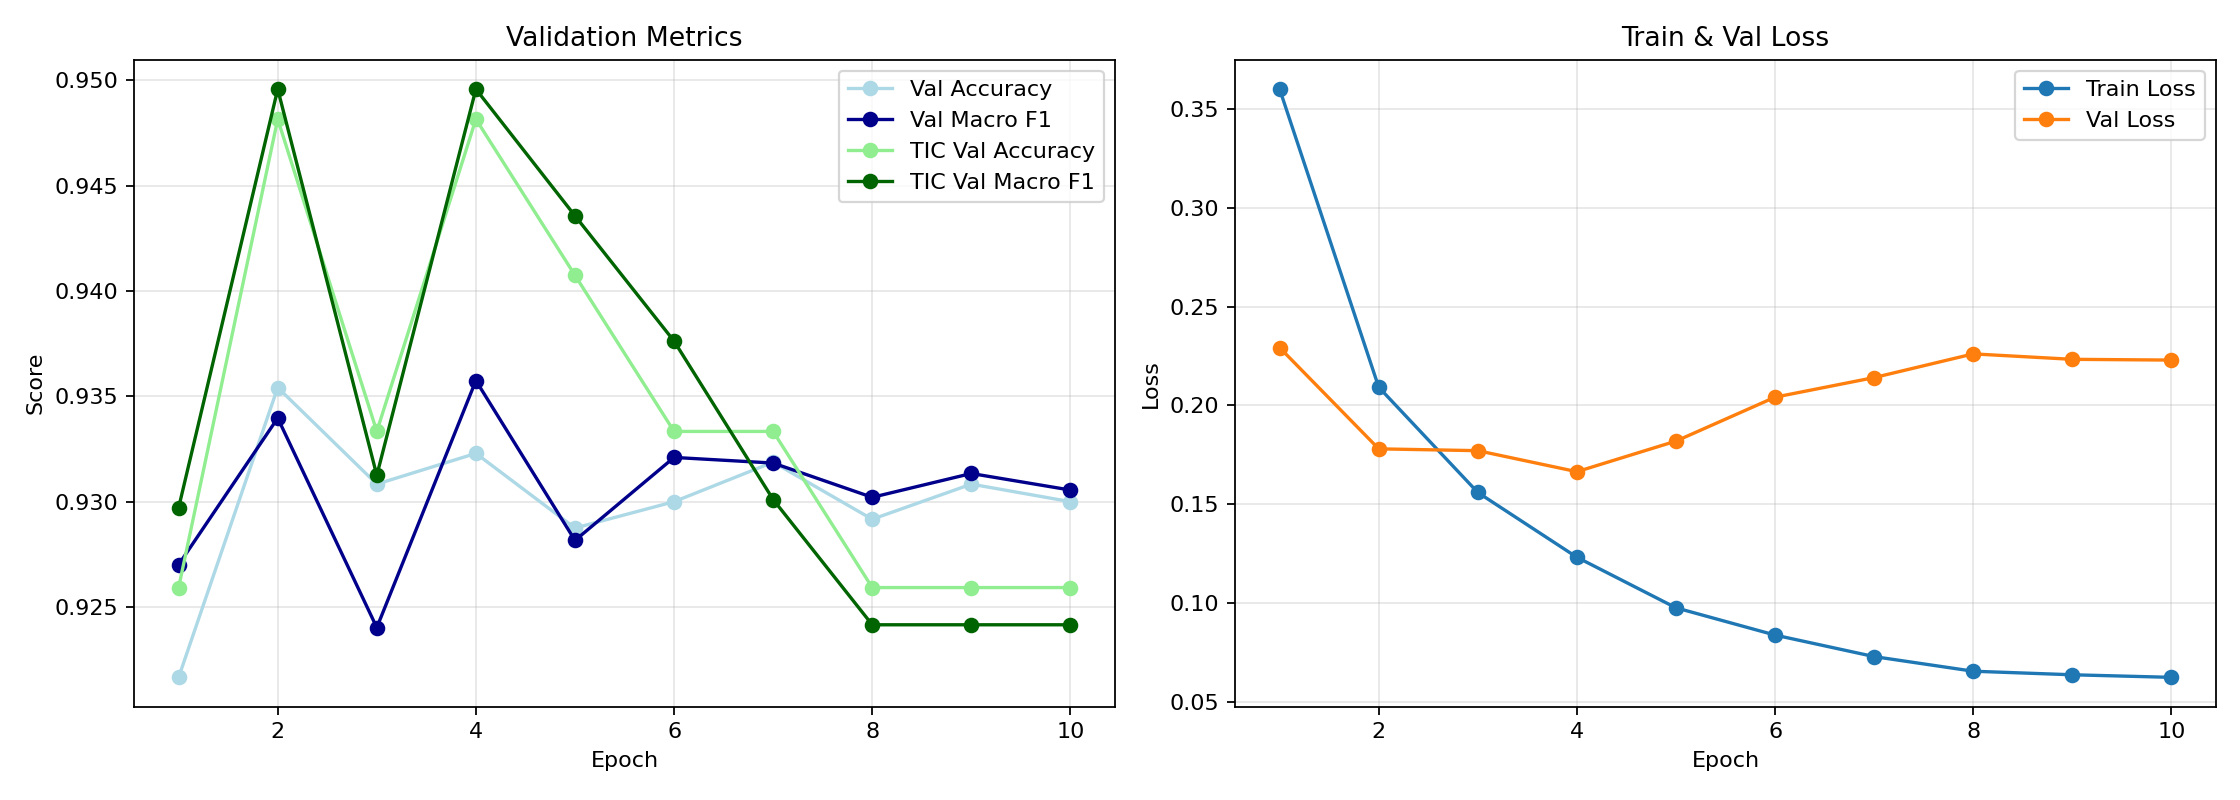
\includegraphics[width=\linewidth]{images/06/phase3_B_chronos_training_curves}
    \caption[Phase 3 -- Chronos-2 Training Curves (B)]{Chronos-2 Training Curves (Task B)}
    \label{fig:06_phase_3_chronos_training_curves_B}
\end{figure}

\FloatBarrier

Training loss again steadily decreased and quickly diverged from the validation loss, after epoch $4$ the validation performance continuously worsened.

\begin{table}[H]
    \centering
    \footnotesize
    \renewcommand{\arraystretch}{1.1}

    \begin{minipage}[t]{0.32\textwidth}
        \centering
        \begin{tabularx}{\textwidth}{X c}
            \toprule
            \textbf{Metric} & \textbf{Score} \tabularnewline
            \midrule
            Accuracy    &  0.9354 \tabularnewline
            Macro F1    & 0.9334 \tabularnewline
            TIC Accuracy & 0.9481 \tabularnewline
            TIC Macro F1 & 0.9496 \tabularnewline
            \bottomrule
        \end{tabularx}
    \end{minipage}
    \hfill
    \begin{minipage}[t]{0.64\textwidth}
        \centering
        \footnotesize
        \begin{tabularx}{\textwidth}{X c c c c c}
            \toprule
            \textbf{Class} & \textbf{Precision} & \textbf{Recall} & \textbf{F1-score} & \textbf{Support} \tabularnewline
            \midrule
            E & 0.94 & 1.00 & 0.97 & 15 \tabularnewline
            P & 0.97 & 0.94 & 0.96 & 81   \tabularnewline
            R & 0.90 & 0.95 & 0.93 & 39   \tabularnewline
            \bottomrule
        \end{tabularx}
    \end{minipage}

    \caption[Phase 3 -- Chronos-2 Validation Metrics (B)]{Chronos-2 Validation Metrics (Task B)}
    \label{tab:06_phase_3_chronos_validation_metrics_B}
\end{table}

\FloatBarrier

The Chronos-2 fine-tune again outperformed the previous best 6-channel transformer.
$\text{Val TIC Macro F1} \approx 0.95$ is a great predictive performance for a dataset of this size.

\subsection{Qwen 2.5 0.5B}

The training took around $180$ and $50$ minutes for tasks A and B respectively.

\subsubsection{Task A}

\begin{figure}[!htbp]
    \centering
    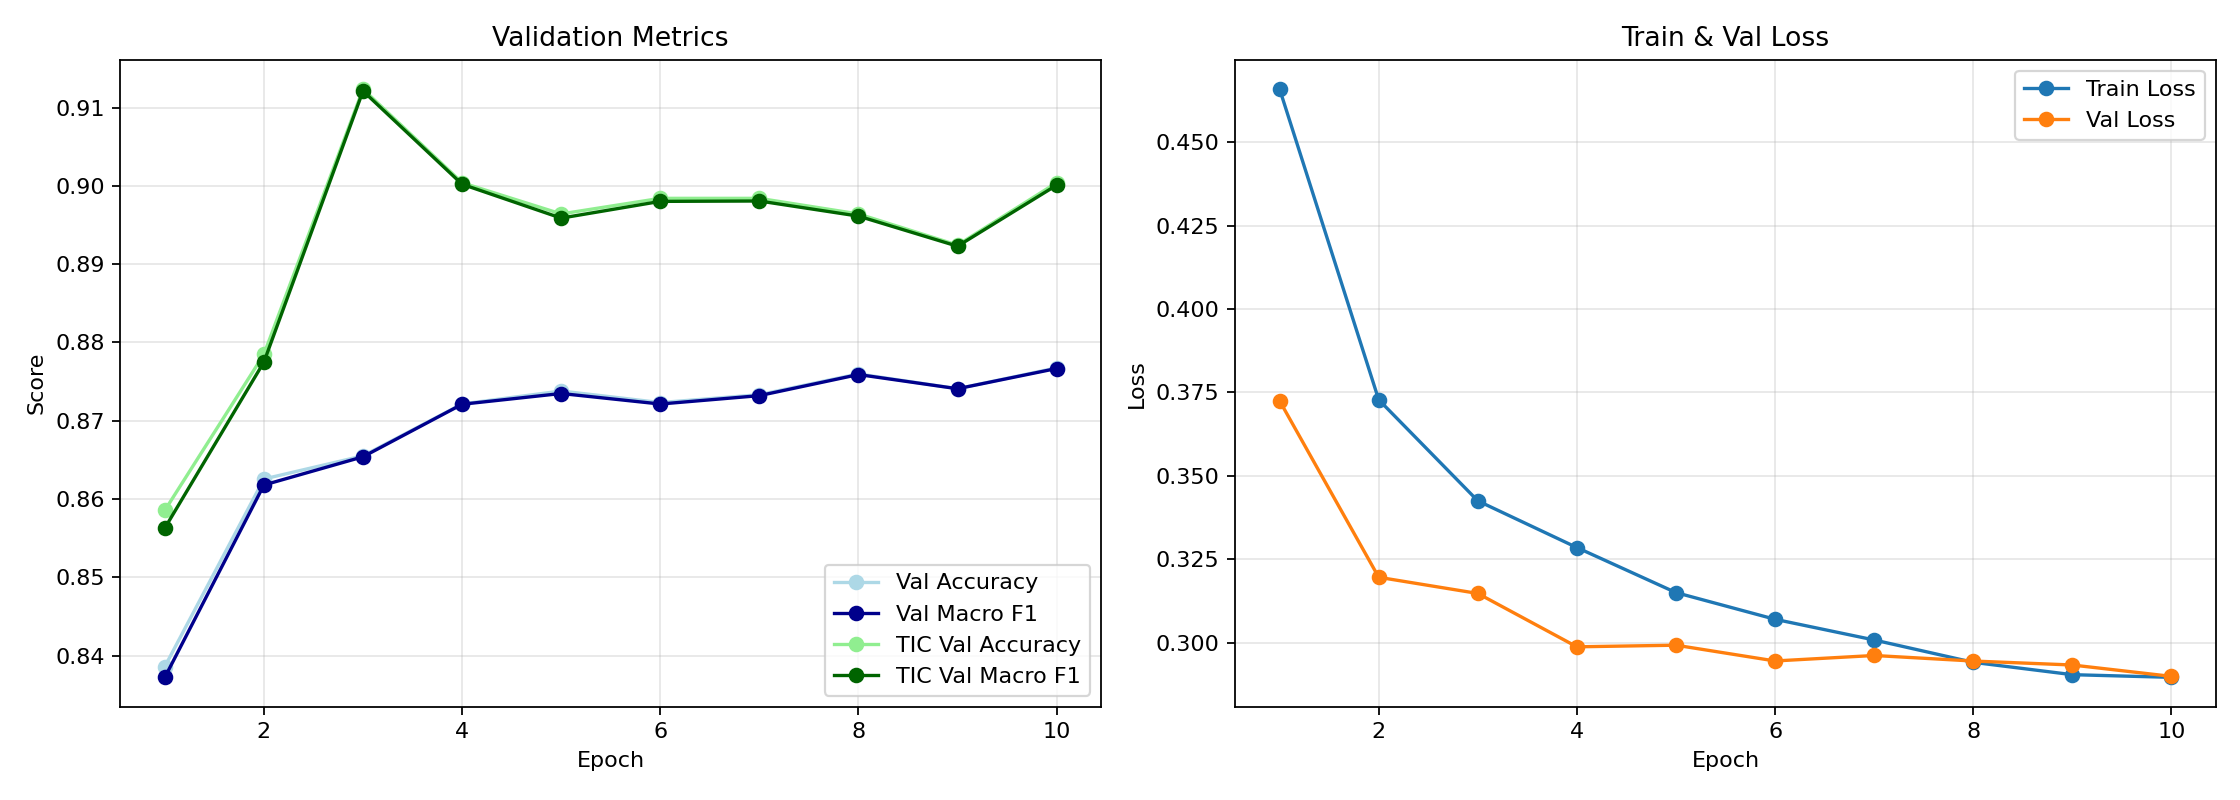
\includegraphics[width=\linewidth]{images/06/phase3_A_qwen_training_curves}
    \caption[Phase 3 -- Qwen 2.5 0.5B Training Curves (A)]{Qwen 2.5 0.5B Training Curves (Task A)}
    \label{fig:06_phase_3_qwen_training_curves_A}
\end{figure}

\FloatBarrier

\begin{table}[H]
    \centering
    \footnotesize
    \renewcommand{\arraystretch}{1.1}

    \begin{minipage}[t]{0.32\textwidth}
        \centering
        \begin{tabularx}{\textwidth}{X c}
            \toprule
            \textbf{Metric} & \textbf{Score} \tabularnewline
            \midrule
            Accuracy    &  0.8655 \tabularnewline
            Macro F1    & 0.8654 \tabularnewline
            TIC Accuracy & 0.9123 \tabularnewline
            TIC Macro F1 & 0.9121 \tabularnewline
            \bottomrule
        \end{tabularx}
    \end{minipage}
    \hfill
    \begin{minipage}[t]{0.64\textwidth}
        \centering
        \footnotesize
        \begin{tabularx}{\textwidth}{X c c c c c}
            \toprule
            \textbf{Class} & \textbf{Precision} & \textbf{Recall} & \textbf{F1-score} & \textbf{Support} \tabularnewline
            \midrule
            N & 0.90 & 0.93 & 0.92 & 259 \tabularnewline
            V & 0.93 & 0.89 & 0.91 & 243   \tabularnewline
            \bottomrule
        \end{tabularx}
    \end{minipage}

    \caption[Phase 3 -- Qwen 2.5 0.5B Validation Metrics (A)]{Qwen 2.5 0.5B Validation Metrics (Task A)}
    \label{tab:06_phase_3_qwen_validation_metrics_A}
\end{table}

\FloatBarrier

\subsubsection{Task B}

\begin{figure}[!htbp]
    \centering
    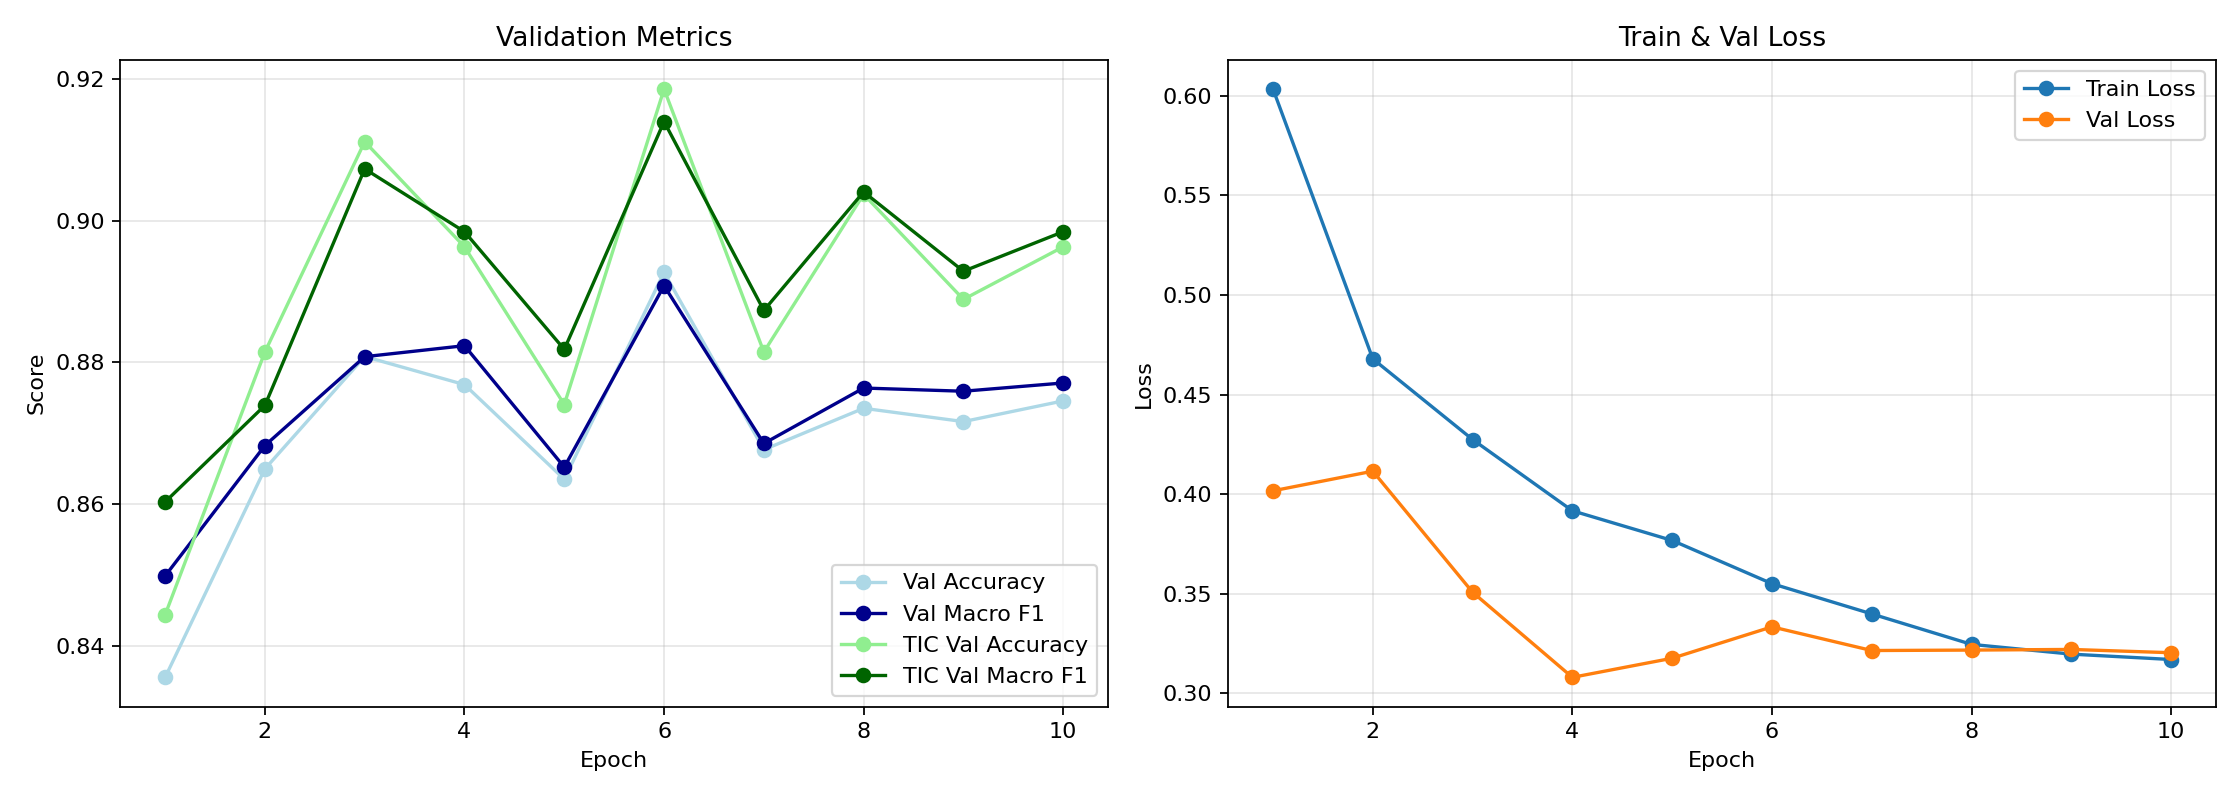
\includegraphics[width=\linewidth]{images/06/phase3_B_qwen_training_curves}
    \caption[Phase 3 -- Qwen 2.5 0.5B Training Curves (B)]{Qwen 2.5 0.5B Training Curves (Task B)}
    \label{fig:06_phase_3_qwen_training_curves_B}
\end{figure}

\FloatBarrier

\begin{table}[H]
    \centering
    \footnotesize
    \renewcommand{\arraystretch}{1.1}

    \begin{minipage}[t]{0.32\textwidth}
        \centering
        \begin{tabularx}{\textwidth}{X c}
            \toprule
            \textbf{Metric} & \textbf{Score} \tabularnewline
            \midrule
            Accuracy    &  0.8927 \tabularnewline
            Macro F1    & 0.8908 \tabularnewline
            TIC Accuracy & 0.9185 \tabularnewline
            TIC Macro F1 & 0.9139 \tabularnewline
            \bottomrule
        \end{tabularx}
    \end{minipage}
    \hfill
    \begin{minipage}[t]{0.64\textwidth}
        \centering
        \footnotesize
        \begin{tabularx}{\textwidth}{X c c c c c}
            \toprule
            \textbf{Class} & \textbf{Precision} & \textbf{Recall} & \textbf{F1-score} & \textbf{Support} \tabularnewline
            \midrule
            E & 1.00 & 0.87 & 0.93 & 15 \tabularnewline
            P & 0.94 & 0.94 & 0.94 & 81   \tabularnewline
            R & 0.85 & 0.90 & 0.88 & 39   \tabularnewline
            \bottomrule
        \end{tabularx}
    \end{minipage}

    \caption[Phase 3 --Qwen 2.5 0.5B Validation Metrics (B)]{Qwen 2.5 0.5B Validation Metrics (Task B)}
    \label{tab:06_phase_3_qwen_validation_metrics_B}
\end{table}

\FloatBarrier

While the Qwen 2.5 0.5B was underfitted and the performance could probably be improved with more epochs, it didn't generalize well enough to justify spending the extensive amounts compute required for more experiments.


\section{Experiment Summary}

We provide a summary of the $16$ experiments showcased in this work.

\begin{table}[H]
    \scriptsize
    \centering
    \renewcommand{\arraystretch}{1.3}
    \begin{tabularx}{\textwidth}{X c@{\hspace{3em}}c@{\hspace{3em}}c}
        \toprule
        \textbf{Task} & \textbf{Model} & \textbf{Architecture}  & \textbf{Val TIC Macro F1}  \tabularnewline \midrule
        \textbf{A} &
        \begin{tabular}{@{}c@{}}
            2-min \\ 8-min \\ 32-min \\ 128-min \\ 4-channel \\ 6-channel \\ \textbf{Chronos-2} \\ Qwen 2.5 0.5B
        \end{tabular} &
        \begin{tabular}{@{}c@{}}
            Transformer \\ Transformer \\ Transformer \\ Transformer \\ Transformer \\ Transformer \\ \textbf{TSFM fine-tune} \\ LLM fine-tune
        \end{tabular} &
        \begin{tabular}{@{}c@{}}
            0.8396 \\ 0.8704 \\ 0.8684 \\ 0.8436 \\ 0.8931 \\ 0.8983 \\ \textbf{0.9261} \\ 0.9129
        \end{tabular} \tabularnewline \midrule
        \textbf{B} &
        \begin{tabular}{@{}c@{}}
            2-min \\ 8-min \\ 32-min \\ 128-min \\ 4-channel \\ 6-channel \\ \textbf{Chronos-2} \\ Qwen 2.5 0.5B
        \end{tabular} &
        \begin{tabular}{@{}c@{}}
            Transformer \\ Transformer \\ Transformer \\ Transformer \\ Transformer \\ Transformer \\ \textbf{TSFM fine-tune} \\ LLM fine-tune
        \end{tabular} &
        \begin{tabular}{@{}c@{}}
            0.6618 \\ 0.8223 \\ 0.8614 \\ 0.9110 \\ 0.9230 \\ 0.9240 \\ \textbf{0.9496} \\ 0.9139
        \end{tabular} \tabularnewline
        \bottomrule
    \end{tabularx}
    \caption[Experiment]{Experiment Summary}
    \label{tab:06_experiment_summary}
\end{table}

\FloatBarrier

As can be seen from \hyperref[tab:06_experiment_summary]{Table 6.21}, the Chronos-2 fine-tunes dominated both tasks, significantly outperforming the other models.


\section{Final Model}

Since the Chronos-2 fine-tune performed the best out of all the evaluated configurations, we used it for more experiments, trying to further optimize the hyperparameters specifically for its architecture and achieve better performance.
However, none of the techniques we tried -- increasing dropout, tuning LoRA values, trying different channel combinations and modifying the fusion head -- lead to any improvement over the original experiment.

The original model proposed in \hyperref[subsubsec:06-chronos]{6.8.1 Chronos-2} was therefore chosen as the final best model.
We use the original checkpoints with the best TIC-level Macro F1 (epoch 5 for Task A and epoch 4 for task B) to evaluate the final model's performance on the test set which should simulate new, unknown data.
The model shouldn't be significantly overfitted on either of those checkpoints, since the training validation loss wasn't increasing yet and the training loss was only slightly lower.

\subsection{Task A Test Evaluation and Discussion}

\begin{table}[H]
    \centering
    \footnotesize
    \renewcommand{\arraystretch}{1.1}

    \begin{minipage}[t]{0.32\textwidth}
        \centering
        \begin{tabularx}{\textwidth}{X c}
            \toprule
            \textbf{Metric} & \textbf{Score} \tabularnewline
            \midrule
            Accuracy    &  0.8702 \tabularnewline
            Macro F1    & 0.8693 \tabularnewline
            TIC Accuracy & 0.8946 \tabularnewline
            TIC Macro F1 & 0.8934 \tabularnewline
            \bottomrule
        \end{tabularx}
    \end{minipage}
    \hfill
    \begin{minipage}[t]{0.64\textwidth}
        \centering
        \footnotesize
        \begin{tabularx}{\textwidth}{X c c c c c}
            \toprule
            \textbf{Class} & \textbf{Precision} & \textbf{Recall} & \textbf{F1-score} & \textbf{Support} \tabularnewline
            \midrule
            N & 0.85 & 0.97 & 0.90 & 259 \tabularnewline
            V & 0.96 & 0.82 & 0.88 & 243   \tabularnewline
            \bottomrule
        \end{tabularx}
    \end{minipage}

    \caption[Final Model Test Metrics (A)]{Final Model Test Metrics (Task A)}
    \label{tab:06_final_model_test_metrics_A}
\end{table}

The test TIC-level Macro F1 went down $\approx 0.02$, this can be expected and is a good generalization performance on a dataset of this size.
It should however be noted that for the \textbf{variable} class the precision increased and recall decreased significantly when compared to the validation metrics.

This behavior has interesting implications for real-world use cases -- for example, the model would be really effective in precisely identifying variable stars, that could be utilized to create large datasets consisting of (mostly) variable stars that could be later used for unsupervised pretraining.
However, the downside is that the model will miss out on some potentially interesting variable stars due to its low recall.

\subsection{Task B Test Evaluation and Discussion}

\begin{table}[H]
    \centering
    \footnotesize
    \renewcommand{\arraystretch}{1.1}

    \begin{minipage}[t]{0.32\textwidth}
        \centering
        \begin{tabularx}{\textwidth}{X c}
            \toprule
            \textbf{Metric} & \textbf{Score} \tabularnewline
            \midrule
            Accuracy    &  0.8998 \tabularnewline
            Macro F1    & 0.8340 \tabularnewline
            TIC Accuracy & 0.9333 \tabularnewline
            TIC Macro F1 & 0.8803 \tabularnewline
            \bottomrule
        \end{tabularx}
    \end{minipage}
    \hfill
    \begin{minipage}[t]{0.64\textwidth}
        \centering
        \footnotesize
        \begin{tabularx}{\textwidth}{X c c c c c}
            \toprule
            \textbf{Class} & \textbf{Precision} & \textbf{Recall} & \textbf{F1-score} & \textbf{Support} \tabularnewline
            \midrule
            E & 0.83 & 0.67 & 0.74 & 15 \tabularnewline
            P & 0.94 & 0.99 & 0.96 & 81   \tabularnewline
            R & 0.94 & 0.93 & 0.94 & 39   \tabularnewline
            \bottomrule
        \end{tabularx}
    \end{minipage}

    \caption[Final Model Test Metrics (B)]{Final Model Test Metrics (Task B)}
    \label{tab:06_final_model_test_metrics_B}
\end{table}

The TIC-level Macro F1 dropped significantly ($\Delta \approx 0.07$) compared to the validation set.
Interestingly, the entire drop in performance was caused by the misclassification of $5$ \textbf{eclipsing} stars as another class which lead to greatly decreased recall and eventually Macro F1 score.

We have investigated the 5 misclassified eclipsing stars and found out that each of them was an interesting non-standard example.

\begin{table}[H]
    \centering
    \small
    \renewcommand{\arraystretch}{1.3}
    \begin{tabularx}{\textwidth}{X c X}
        \toprule
        \textbf{TIC} & \textbf{Eclipsing Subclass} & \textbf{Note} \tabularnewline
        \midrule
        224595426 & EA & Extremely noisy, the eclipses are not easily identifiable. \tabularnewline
        229710150 & ELL & Peaks are not sharp -- similar to a rotating star. \tabularnewline
        259238257 & ELL & Peaks are not sharp -- similar to a rotating star. \tabularnewline
        288346083 & EA & Atypically long period -- the eclipse happened only once per 50 days. \tabularnewline
        362226108 & EW & Very similar to a pulsating star. \tabularnewline
        \bottomrule
    \end{tabularx}
    \caption[Missclassified Eclipsing Stars]{Misclassified Eclipsing Stars}
    \label{tab:06_misclassified_eclipsing_stars}
\end{table}

\begin{figure}[!htbp]
    \centering
    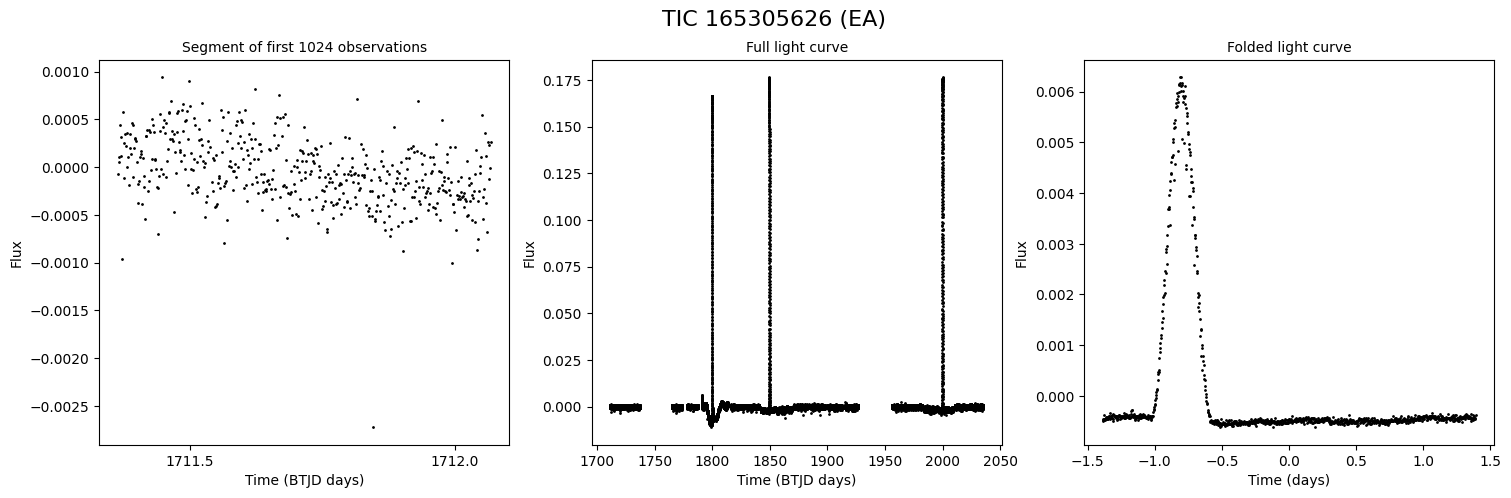
\includegraphics[width=\linewidth]{images/06/long_period_star}
    \caption[Long Period EA Star]{TIC 288346083, a misclassified eclipsing star with atypically long period.}
    \label{fig:06_long_period_star}
\end{figure}

Despite the worse performance on the \textbf{eclipsing} class, the model has generalized well on the remaining 2 classes, their test metrics being nearly identical to the validation metrics.


\section{Computational Performance}

For usage on large real-world datasets, the model must be able to efficiently process large volumes of data (millions of light curves).
We provide a brief analysis of the model's processing speed using available data.

There are 2 main possible bottlenecks:

\begin{itemize}
    \item \textbf{Preprocessing}
    \item \textbf{Inference}
\end{itemize}

\subsection{Preprocessing}

The preprocessing speed was $\approx 13.8 \, \text{light curves/s}$ on AMD Ryzen 5 9700X CPU when utilizing all 8 cores or around \num{1200000} light curves per day.
While the preprocessing pipeline could certainly be optimized, it would probably not achieve more than $10\times$ speedup.

\subsection{Inference}

Information from the training logs shows that model took $10.7$ seconds to run evaluation on the val subset of $135$ light curves, making the inference speed $\approx 12.6 \, \text{light curves/s}$ or around \num{1100000} on an AMD Radeon RX9070 GPU.

\subsection{Summary}

With the available information, we can conclude that the pipeline is theoretically capable of analyzing up to millions of light curves in reasonable time (days) on higher end consumer-grade hardware.
The processing speed could be further increased by utilizing industrial-grade GPU clusters and more parallelization.